% !TEX encoding = UTF-8 Unicode
\documentclass[fleqn,twoside,dvipsnames]{article}
\usepackage[ngerman]{babel}
\usepackage[utf8]{inputenc}
\usepackage[T1]{fontenc}
\usepackage{amsmath}
\usepackage{amssymb}
\usepackage{booktabs}
\usepackage{calligra}
% for adjustwidth environment
\usepackage[strict]{changepage}
\usepackage{cite}
\usepackage{comment}
\usepackage{csquotes}
\usepackage{enumitem}
%\usepackage{eurosym}
\usepackage{fancyhdr}
\usepackage{fdsymbol}
\usepackage{float}
\usepackage{framed}
\usepackage{graphicx}
\usepackage{marvosym}
\usepackage{mathtools}
\usepackage{multirow}
\usepackage{nicefrac}
\usepackage[normalem]{ulem}
\usepackage{pdfpages}
\usepackage{pifont}
\usepackage{romanbar}
\usepackage{siunitx}
\usepackage{stanli}
\usepackage{svg}
\usepackage{tabto}    
\usepackage{tabularx}
\usepackage{textcomp}
\usepackage{tikz}
\usepackage{titlesec}
\usepackage{todonotes}
\usepackage{wasysym}
\usepackage{wrapfig}
\usepackage{xcolor}
\usepackage{yfonts}
%\usepackage{3dstructuralanalysis}
%\usepackage{emerald}
%\usepackage{structuralanalysis}
%\usepackage{units}

\setlength{\headheight}{12.51453pt}

%special braces after itemize
\usepackage{tikz}
\usetikzlibrary{decorations.pathreplacing,calc}
\newcommand{\ntikzmark}[2]{#2\thinspace\tikz[overlay,remember picture,baseline=(#1.base)]{\node[inner sep=0pt] (#1) {};}}

\newcommand{\makebrace}[3]{%
    \begin{tikzpicture}[overlay, remember picture]
        \draw [decoration={brace,amplitude=0.5em},decorate]
        let \p1=(#1), \p2=(#2) in
        ({max(\x1,\x2)}, {\y1+0.8em}) -- node[right=0.6em] {#3} ({max(\x1,\x2)}, {\y2});
    \end{tikzpicture}}


%shorther tab 
\newcommand\mytab{\tab \hspace{-2.5cm}}

% Framed quote
        \definecolor{formalshade}{rgb}{0.95,0.95,1}
\newenvironment{formal}{%
        \def\FrameCommand{\hspace{1pt} {\color{lightgray}\vrule width 2pt}  {\color{formalshade}\vrule width 4pt} \colorbox{formalshade} }%
        \MakeFramed{\advance\hsize-\width\FrameRestore}\noindent\hspace{-4.55pt}% disable indenting first paragraph
        \begin{adjustwidth}{}{7pt}\vspace{2pt}\vspace{2pt}}
        {\vspace{2pt}\end{adjustwidth}\endMakeFramed }

%Befehle abändern
%Itemize ohne Lücken
\setlist[itemize]{noitemsep, topsep=2pt}
\raggedbottom
%\renewcommand{\todo}[1]{\todo[inline]{#1}}


%Betragsfunktion
\newcommand{\abs}[1]{\ensuremath{\left\vert#1\right\vert}}
%Einheitenfunktion
\newcommand{\un}[2]{{\unit[#1]{\color{black!100}[#2]}}}

\usepackage[pdftex, colorlinks, linkcolor=black, frenchlinks]{hyperref}
\usepackage[a4paper , lmargin = {2.5cm} , rmargin = {2cm} , tmargin = {2.5cm} , bmargin = {2.5cm} ]{geometry}
\pagestyle{fancy}

\title{\Huge{\textfrak{Bauen im Bestand \& Energetische Sanierung}}}
\author{\calligra{Jonas Konrad}}
\date{\textfrak{\today}}

\begin{document}
\parindent 0pt
\fancyhead[L]{Jonas Konrad}
\fancyfoot[L]{\frakfamily J. K.}
\fancyfoot[R]{\frakfamily }
\fancyfoot[C]{\frakfamily Kapitän ich schweife kurz 90 Minuten ab und sein energetisch überforderter Gehilfe \\Seite \thepage}
\maketitle \thispagestyle{empty}
%\initfamily %Für Initialien
\begin{center}
\textfrak{Diese Sammlung der Vorlesungsinhalte wurde im Wintersemester 2022/23 von Jonas Konrad verfasst.\\BiB: Dr.-Ing. Harald Schneider , ES: M.Sc. Tobias Kropp\\Kein Anspruch auf Vollständigkeit oder Fehlerfreiheit.\\LaTex Vorlage: github.com/Neowise33}
\end{center}
\tableofcontents
%\listoftodos
\newpage

%\listoftodos
%\newpage



\section{Einführung} 
        \label{BiB-Zahlen/Fakten}
    \subsection{Daten zum Gebäudebestand} 
        \begin{itemize}
            \item Die Zukunft des Bauens liegt im Bestand: 75\% der in 2020 benötigten Gebäudesubstanz waren 2010 bereits vorhanden
                \item $\frac13$ der Bauwerke sind oberirdisch sichtbar, $\frac23$ unterirdisch (Rohre,Gründungen)\\
                        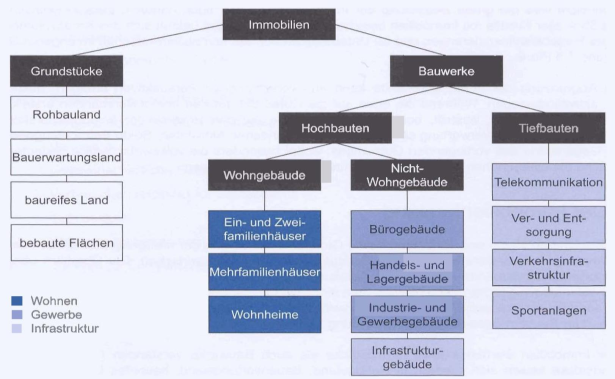
\includegraphics[width=0.9\textwidth]{Grafiken/Einführung/Ueberblick Immobilien.png}
                \item Bruttobauanlagevermögen: 2010: 11,3 Bil.€ $\rightarrow$ 2019: 16,9 Bil.€\\
                        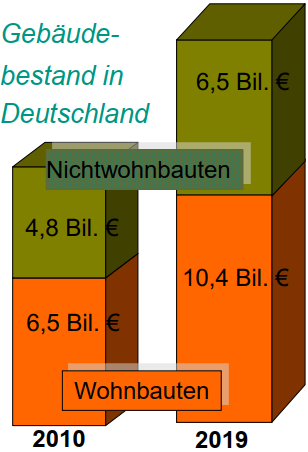
\includegraphics[width=0.2\textwidth]{Grafiken/Einführung/Gebaeudebestand.png}
                \item Altersverteilung: über 25\% des Wohnungsbestands in Deutschland wurde vor 1948 erstellt
                \item Bauvermögen nach Sektoren: (Größenordnungen wichtig) \label{Bauvermögen}\\
                        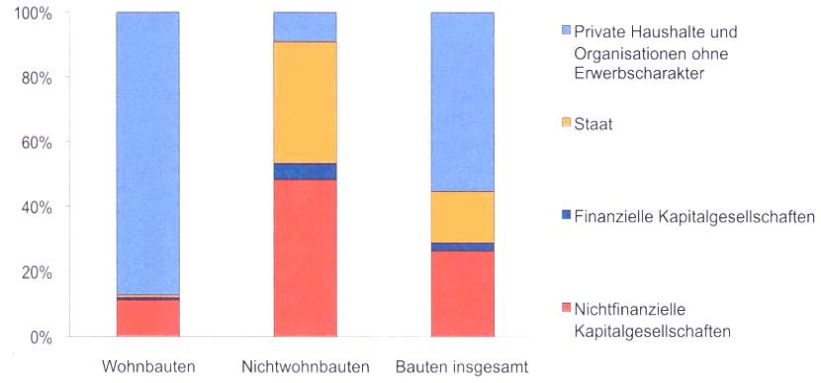
\includegraphics[width=0.5\textwidth]{Grafiken/Einführung/Bauvermoegen nach Sektoren.png}\\
                        Insgesamt: Privat: 55\% Kapitalgesellschaften: 30\% Staat: 15\%\\
            \begin{minipage}{0.5\textwidth}
                \item Baugenehmigungen und Baufertigstellungen \\von Wohnungen\\
                        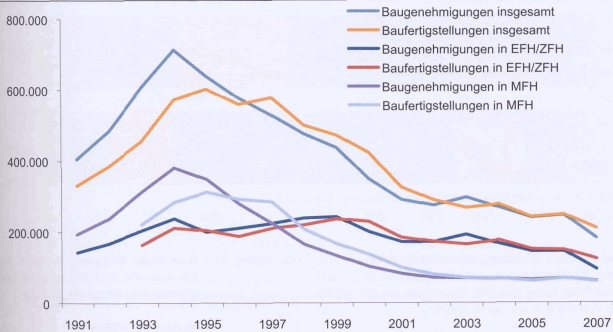
\includegraphics[width=0.9\textwidth]{Grafiken/Einführung/Baugenehmigungen von Wohnungen.png}
                \item Fertiggestellte Wohnungen je 10.000 Einwohner \\1950 bis 2007\\
                        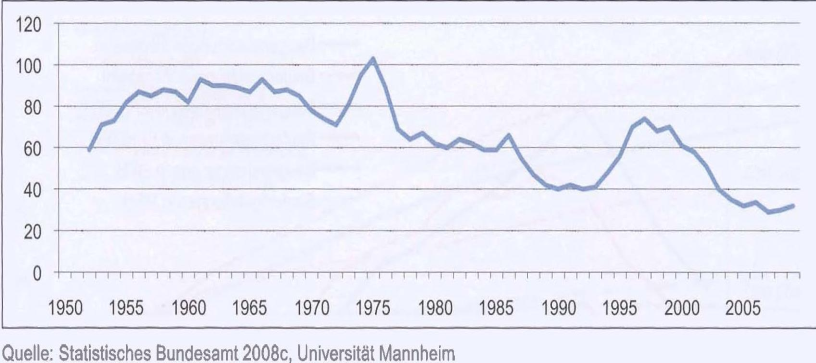
\includegraphics[width=0.9\textwidth]{Grafiken/Einführung/Fertiggestellte Wohnungen je 10.000 Einwohner 1950 bis 2007.png}
                \item Wohnungsgröße in qm nach Baujahr\\ der Wohngebäude 2006 in \%\\
                        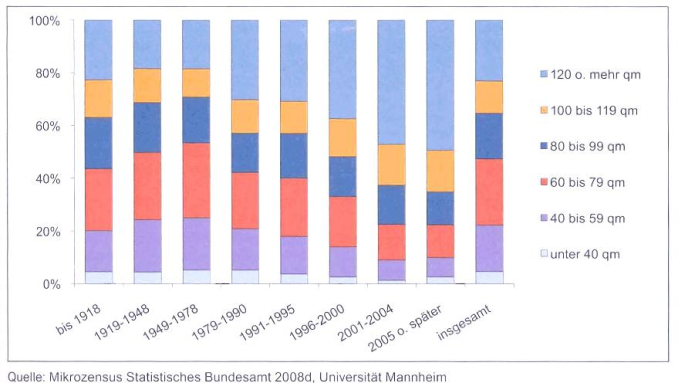
\includegraphics[width=0.9\textwidth]{Grafiken/Einführung/Wohnungsgroesse in qm nach Baujahr der Wohngebaeude 2006.png}
            \end{minipage}
            \begin{minipage}{0.5\textwidth}
                \item Entwicklung des Wohnungsbauvolumen 2003-2020\\
                        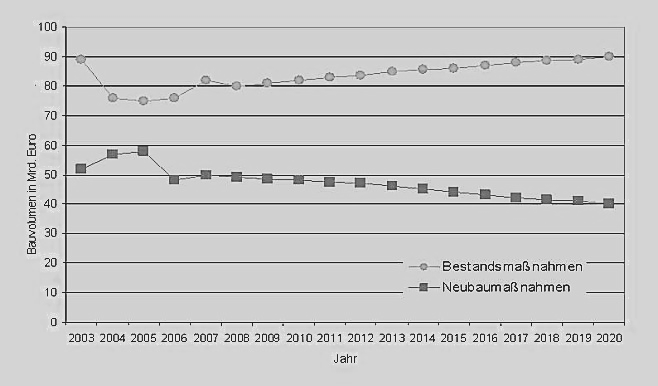
\includegraphics[width=0.9\textwidth]{Grafiken/Einführung/Entwicklung Wohnungsbauvolumen 2003-2020.png}
                \item Wohnungen: Fertigstellungen pro 10.000 Einwohner\\
                        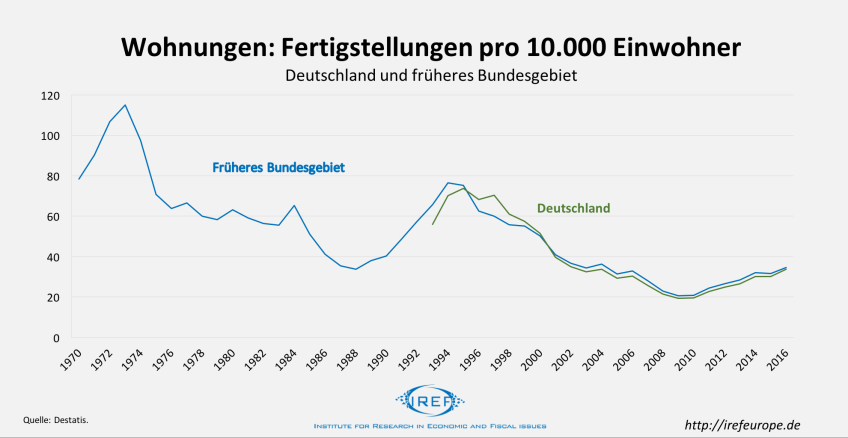
\includegraphics[width=0.9\textwidth]{Grafiken/Einführung/Wohnungen Fertigstellungen pro 10.000 Einwohner.png}
                \item Daten zum Gebäudebestand\\
                    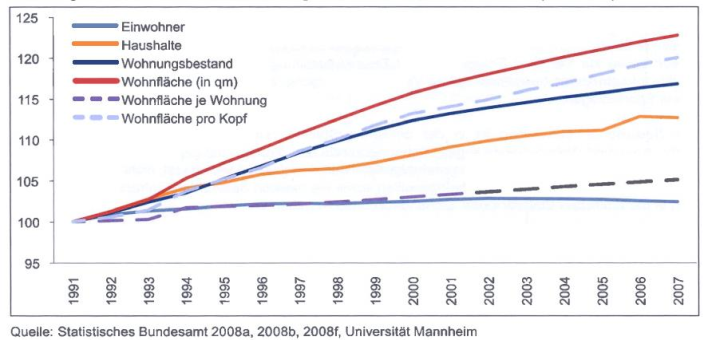
\includegraphics[width=0.93\textwidth]{Grafiken/Einführung/Daten zum Gebaeudebestand.png}
            \end{minipage}
        \end{itemize}
                        
    \subsection{Wirtschaftliche Bedeutung von Bestandsbauten}
        \begin{itemize}
            \item Kommunaler Investitionsbedarf 2006-2020: 704 Mrd. € (basierend auf Preisen von 2000)\\
                    $\rightarrow$ 47 Mrd. € / Jahr
            \item Davon gehen insgesamt:
                \begin{itemize}
                    \item 162 Mrd. € in den Straßenbau
                    \item 73 Mrd. € in Ausbau von Schulen
                    \item 58 Mrd. € in kommunale Abwasseranlagen
                    \item 35 Mrd. € in Sportstätten
                    \item 31 Mrd. € in Krankenhäuser
                    \item 20 Mrd. € in Verwaltungsgebäude
                \end{itemize}
                $\Rightarrow$ ca. 23\% in Gebäudebau/-sanierung
            \newpage
            \item Maß für Alterungsprozess des Anlagevermögens: Modernitätsgrad\\
                        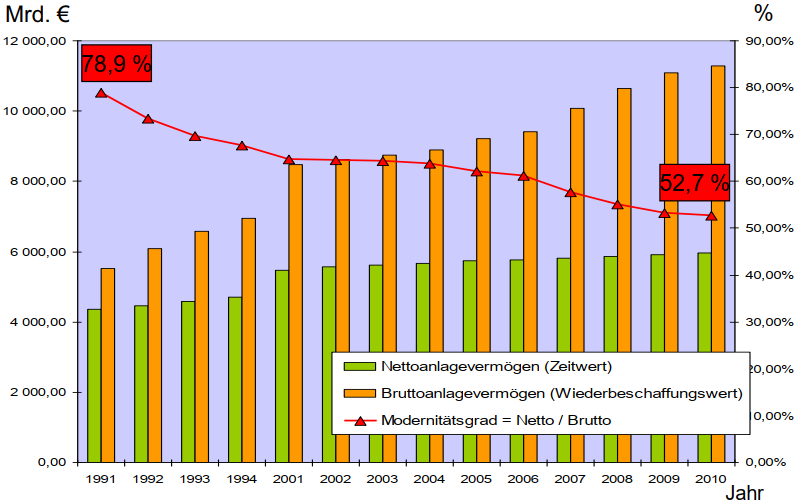
\includegraphics[width=0.55\textwidth]{Grafiken/Einführung/Modernitaetsgrad Anlagevermoegen.png}
            \item Gebäudebestand braucht umfassende, zunehmend komplexe Instandhaltung
            \item Ausbildungssituation
                \begin{itemize}
                    \item Baubestand als kulturelle und volkswirtschaftliche Größe wurde bisher nicht klar erkannt.
                    \item Auch die Bedeutung des Baubestands in der Öffentlichkeit wurde nicht richtig wahrgenommen.
                    \item Geringe Kenntnisse über den Baubestand. \\
                    Daher keine vorausschauenden Strategien zur Durchführung von Instandsetzungs- und Modernisierungsmaßnahmen
                    \item $\rightarrow$ „Schlechte“ Ausbildung der Planer und Ausführenden, sowohl im Hinblick auf die Diagnose als auch im Hinblick auf die Konzeption und Ausführung von Maßnahmen.
                \end{itemize}
            \item Trendwende in der europäischen Bauindustrie: \enquote{Die Zukunft des Bauens liegt im Bestand Ifo-Institut konstatiert eine Trendwende in der europäischen Bauindustrie}
        \end{itemize}

    \subsection{Wandel der Bauindustrie} \label{Entwicklung Baubranche}
        \begin{itemize}
            \item Die neue Wertschöpfungskette\\
                    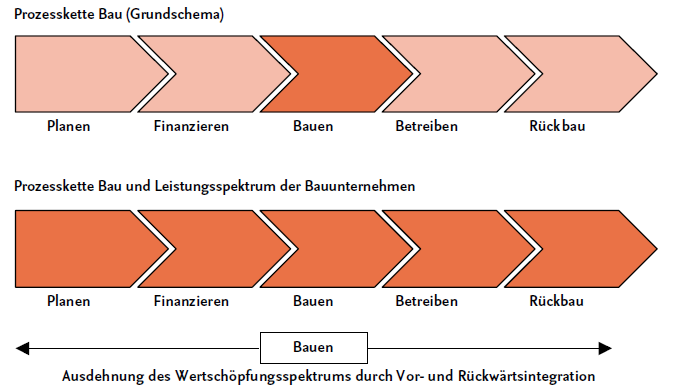
\includegraphics[width=0.65\textwidth]{Grafiken/Einführung/Neue Wertschoepfungskette.png}
            \item Beispiel Bilfinger: Anteil der Dienstleistungen an der Konzernleistung\\
                    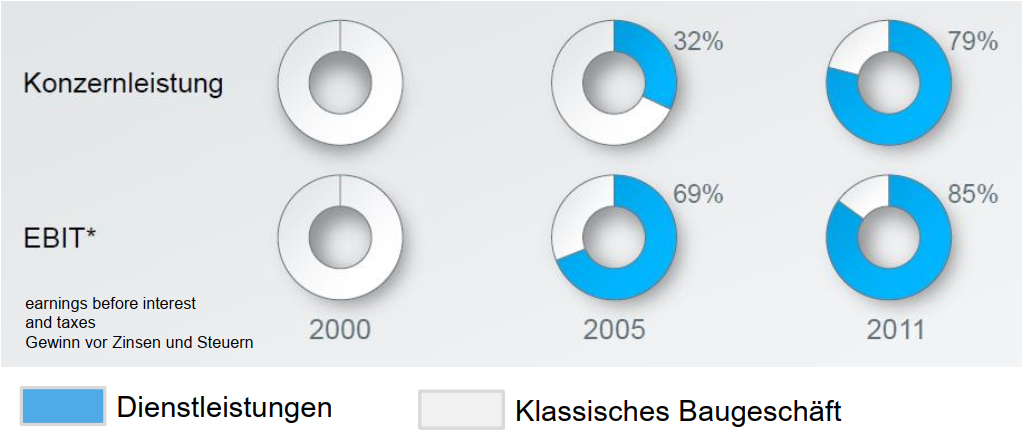
\includegraphics[width=0.45\textwidth]{Grafiken/Einführung/Wandel Beispiel Bilfinger.png}
                    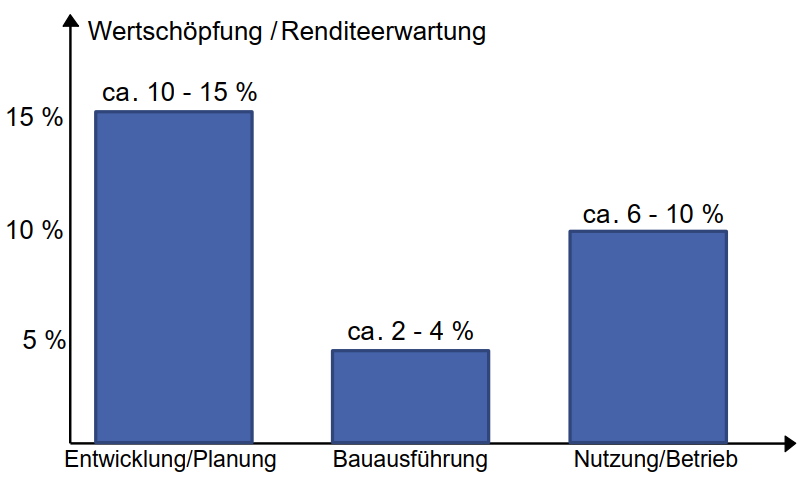
\includegraphics[width=0.45\textwidth]{Grafiken/Einführung/Bilfinger Renditeerwartung.png}
           \newpage
            \item Profilschärfung in Richtung Services durch Unternehmensankäufe\\
                    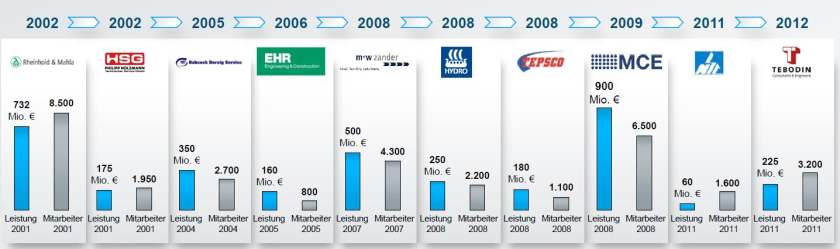
\includegraphics[width=0.65\textwidth]{Grafiken/Einführung/Bilfinger Unternehmensankaeufepng.png}
            \item Höhere Margen im Servicegeschäft\\
                    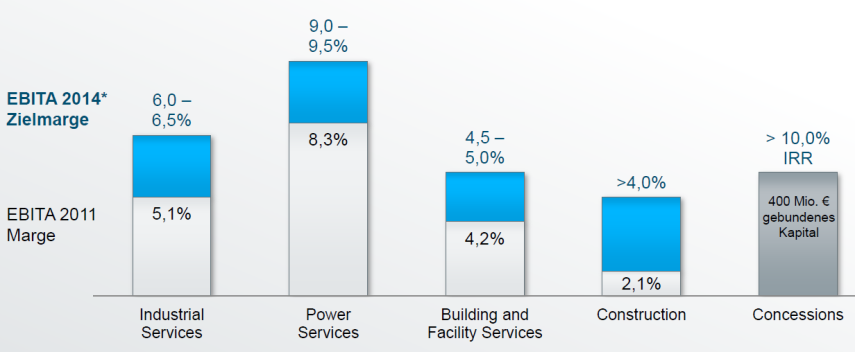
\includegraphics[width=0.65\textwidth]{Grafiken/Einführung/Bilfinger Margen.png}
        \end{itemize}

    \subsection{Bedeutung in Forschung und Lehre}
        \begin{itemize}
            \item Forschung nach regionaler Verteilung:
                \begin{itemize}
                    \item Schwerpunkt der Forschung in GB und Nordeuropa
                    \item Vereinzelte Vorhaben in Zentraleuropa
                    \item Vereinzelte Vorhaben in Asien und Australien/Neuseeland
                \end{itemize}
        \end{itemize}

    \subsection{Verständnisfragen zu Themenabschnitt}
        \begin{itemize}
            \item Wie viel Prozent des deutschen Wohnungsbestandes wurde vor 1948 errichtet? (Stand 2007)\\
                    $\rightarrow$ ca. $28 \%$
            \item Aus welchen Gründen vollziehen die „klassischen B Bauunternehmen einen Wandel zum ganzheitlichen Baudienstleister mit Leistungen in allen Lebenszyklusphasen eines Bauwerks?\\
                    $\rightarrow$ 1. Rückläufige Neubauinvestitionen 2. höhere Gewinnmargen
            \item In welcher Phase des Gebäudelebenszyklus lassen sich it. Bilfinger (2012) die höchsten Margen erzielen?\\
                    $\rightarrow$ Projektentwicklung / Projektplanung
        \end{itemize}
      
\newpage
        
\section{Instandhaltung: Definition und Strategien}

    \subsection{Theoretische Grundlagen}
        \begin{itemize}
            \item Erstes Instandhaltungsgesetz v. König Magnus ”the Lawmaker” 1278. Das Gesetz legt fest:
                \begin{itemize}
                    \item Wer verantwortlich ist
                    \item Was wie oft zu tun ist
                \end{itemize}
            \item Vorkehrungen um die Lebensdauer zu erhöhen:
                \begin{itemize}
                    \item Materialien mit hoher Qualität
                    \item ausgeprägte Bauart zur Verbesserung der Haltbarkeit
                    \item ausgebildete Handwerker
                    \item Wissen über Umweltverträglichkeit
                    \item vorbeugende Instandhaltung
                \end{itemize}
            \item Wie ist Instandhaltung definiert?
                \begin{itemize}
                    \item Modernisieren $\rightarrow$ Funktion kann sich verändern
                    \item Verbessern $\rightarrow$ Abnutzungsvorrat über Vorheriges Maß erhöht, ohne Änderung der Funktion
                    \item Anpassung
                    \item Erhaltung
                    \item Erneuern
                    \item Erweitern
                    \item Instandsetzung
                    \item Renovieren
                    \item Reparieren
                    \item Restaurieren
                    \item Revitalisieren
                    \item Sanieren
                    \item Umbauen
                    \item Unterhalten
                    \item Wartung
                    \item Werterhaltung
                \end{itemize}
            \item Normen, Richtlinien und Verordnungen zur Instandhaltung:\\
                    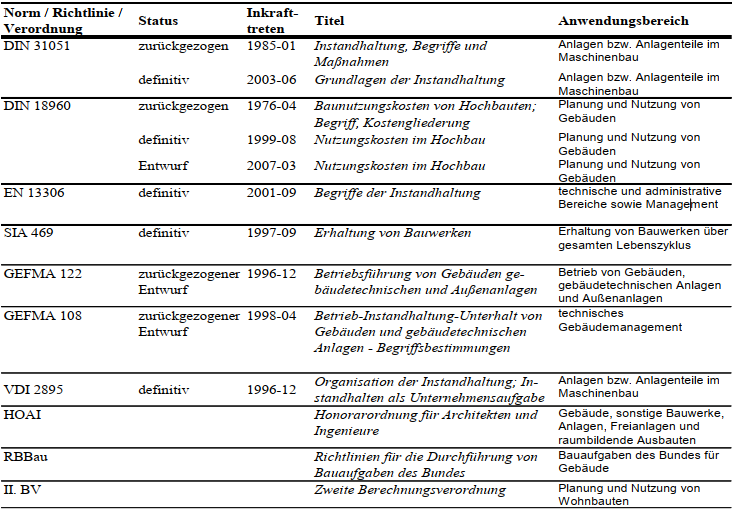
\includegraphics[width=0.45\textwidth]{Grafiken/Instandhaltung/Normen Uebersicht.png}
            \item Kommunikationsproblem Instandhaltung:\\
                    Zuwachs von Fachvokabular $\rightarrow$ Begriffsverwechslungen $\rightarrow$ Verständigungsprobleme
            \item Definition Instandhaltung nach DIN 31051:2012-09 / Grundlagen der Instandhaltung:\\
                    \begin{tabular}{|p{13cm}}\enquote{Kombination aller technischen und administrativen Maßnahmen sowie Maßnahmen des Managements während des Lebenszyklus einer Einheit, die dem Erhalt oder der Wiederherstellung ihres funktionsfähigen Zustands dient, sodass sie die geforderte Funktion erfüllen kann.} \end{tabular}\vspace{1.5mm}\\
            \item Definition nach DIN 31051:2003-06 / Grundlagen der Instandhaltung: \label{DIN31051}\\
                    Anwendungsbereiche: 
                        \begin{itemize}
                            \item Kostengruppe 300 (Baukonstruktionen)
                            \item Kostengruppe 400 (Technische Anlange)
                        \end{itemize}
                        
                        \resizebox{0.9\textwidth}{!}{
                        \begin{tabular}{|c|c|c|c}\hline
                        \multicolumn{4}{|c|}{\textbf{Instandhaltung}} \\ \hline
                        \multicolumn{1}{|c|}{Wartung} & \multicolumn{1}{c|}{Inspektion} & \multicolumn{1}{c|}{Instandsetzung} & \multicolumn{1}{c|}{Verbesserung} \\ \hline
                        \multicolumn{1}{|c|}{\begin{tabular}[c]{@{}c@{}}Verzögerung des \\ Abbbaus des \\ vorhandenen Abnutzungsvorrats\end{tabular}} & \multicolumn{1}{c|}{\begin{tabular}[c]{@{}c@{}}Feststellung und \\ Beurteilung des \\ Ist-Zustands\end{tabular}} & \multicolumn{1}{c|}{\begin{tabular}[c]{@{}c@{}}Rückführung in den \\ funktionsfähigen Zustand\\ $\rightarrow$ es funktioniert noch, \\ aber ich erhöhe den\\ Abnutzungsvorrat\end{tabular}} & \multicolumn{1}{c|}{\begin{tabular}[c]{@{}c@{}}Steigerung der \\ Funktionssicherheit \\ (ohne Funktionsänderung)\end{tabular}} \\ \hline
                        \multicolumn{3}{c}{ $\overset{ \underbracket[1pt][3pt]{\phantom{\text{Der Text hier ist nur als Lückenfüller gedacht, damit die Klammer lang genug ist}}} }{\text{ursprünglicher Abnutzungsvorrat}} $} & 
                        \end{tabular} }
    
            \item Begriffe nach DIN 31051:2012-9
                \begin{itemize}
                    \item Wartung:\\
                        \begin{tabular}{|p{13cm}} \enquote{Maßnahmen zur Verzögerung des Abbaus des vorhandenen Abnutzungsvorrats} \end{tabular}\vspace{1.5mm}\\
                        Präventivmaßnahme, die durch regelmäßige Pflege in Form von Reinigungs-, Schmier-, Konservierungs- und kleineren Reparaturarbeiten einer vorzeitigen Abnutzung der Anlagen vorbeugt und deren Funktionsfähigkeit erhält.\\
                        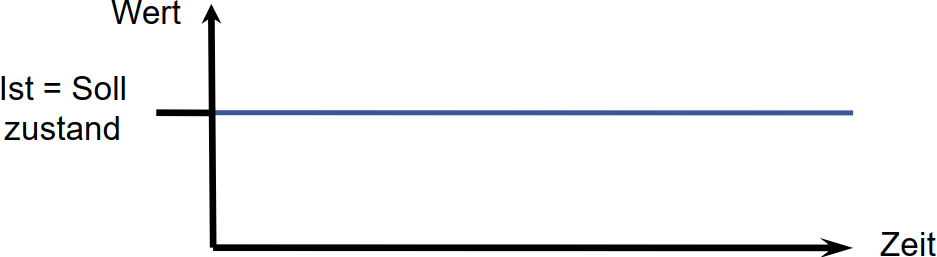
\includegraphics[width=0.45\textwidth]{Grafiken/Instandhaltung/Wartung.png}
                    \item Inspektion:\\
                        \begin{tabular}{|p{13cm}} \enquote{Maßnahmen zur Feststellung und Beurteilung des Istzustandes einer Einheit einschließlich der Bestimmung der Ursachen der Abnutzung und dem Ableiten der notwendigen Konsequenzen für ein künftige Nutzung} \end{tabular}\vspace{1.5mm} \\ 
                        Inspektion ist ein vorbeugende Maßnahme. Sie dient der Feststellung und Beurteilung des Ist-Zustandes, um Zustandsverschlechterungen und Schäden frühzeitig zu erkennen und entsprechende Gegenmaßnahmen einleiten zu können.
                    \item Instandsetzung:\\
                        \begin{tabular}{|p{13cm}} \enquote{Physische Maßnahme, die ausgeführt wird, um die Funktion einer fehlerhaften Einheit wiederherzustellen} \end{tabular}\vspace{1.5mm}\\
                        Beseitigung von baulichen Mängel, um die Gebäudesubstanz vor einem weiteren Verlust zu bewahren. Zeitpunkt der Investition vom Zustand der Immobilie bestimmt. Verschieben erhöht die Geldausgabe. Es besteht Handlungsbedarf.
                    \item Verbesserung:\\
                        \begin{tabular}{|p{13cm}} \enquote{Kombination aller technischen und administrativen Maßnahmen sowie Maßnahmen des Managements zur Steigerung der Zuverlässigkeit und/oder Instandhaltbarkeit und/oder Sicherheit einer Einheit, ohne ihre ursprüngliche Funktion zu ändern} \end{tabular}\vspace{1.5mm}
                \end{itemize}
            \item Abbau des Abnutzungsvorrats: \label{BiB-Abnutzungsvorrat}\\
                    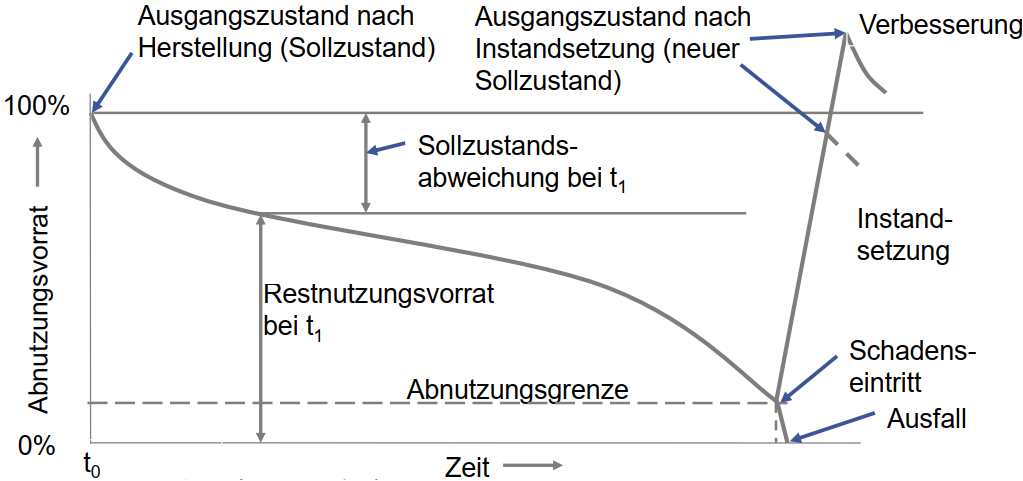
\includegraphics[width=0.45\textwidth]{Grafiken/Instandhaltung/Abbau des Abnutzungsvorrats.png}\\
                    Anfangs schnelle Abnutzung und bei leichten Schäden höhere Folgeschäden, ähnliche Wertverfall wie bei Auto, Instandsetzung kann auch vor Schadenseintritt greifen
            \item SIA 469: Erhaltung von Bauwerken (1997):\\
                \begin{tabular}{|p{13cm}} Ziel des SIA 469: \enquote{… bezweckt die fachgerechte und wirtschaftliche Erhaltung von Bauwerken unter der Berücksichtigung ihres kulturellen Werts. Zum Bauwerk gehören das Tragwerk, die Gebäudehülle, der Ausbau und die technischen Anlagen (z.B. Haustechnik).} \end{tabular}\vspace{1.5mm}\\
                \begin{tabular}{|p{13cm}} Bauwerkserhaltung nach SIA 469: \enquote{Gesamtheit der Tätigkeiten und Maßnahmen zur Sicherstellung des Bestandes sowie der materiellen und kulturellen Werte eines Bauwerks. Die Bauwerkserhaltung ist der bauspezifische Teil der Bauwerksbewirtschaftung. Sie beginnt nach erfolgter Inbetriebnahme eine Bauwerkes und erstreckt sich über dessen gesamte Nutzungsdauer.} \end{tabular}\vspace{1.5mm}\\
            \item DIN EN 13306: Begriffe der Instandhaltung (2017):\\
                \begin{tabular}{|p{13cm}} DIN EN 13306:2001-09: \enquote{Der Zweck dieser europäischen Norm ist die Definition der Grundbegriffe für alle Instandhaltungsarten und für das Instandhaltungsmanagement, unabhängig von der betrachten Einheit, mit Ausnahme von Software.} \end{tabular}\vspace{1.5mm}\\
                \begin{tabular}{|p{13cm}} Anwendungsbereich der DIN EN 13306:2001-09: \enquote{Diese europäische Norm legt die Grundbegriffe und Definitionen für alle technischen und administrativen Bereiche sowie den Managementbereich der Instandhaltung fest.} \end{tabular}\\
                \begin{itemize}
                    \item Entwurf 2008-10 $\rightarrow$ Überarbeitung und Anpassung an den Stand der Technik
                    \item dient als Übersetzungshilfe bei länderübergreifenden Instandhaltungsdienstleistungen und instandzuhaltenden Anlagen
                    \item gibt keine Strukturierung der Instandhaltung vor, nur Begriffserklärung
                    \item Wird spezifischen Anforderungen der einzelnen Länder nicht gerecht, z.B. Abnutzung (Deutschland)
                    \item Dient meist als Ergänzung der nationalen Normen (z.B. SIA oder DIN)
                \end{itemize}
            \item GEFMA 122 „Betriebsführung von Gebäuden, gebäudetechnischen und Außenanlagen“ \\Praxisanforderung:
                \begin{itemize}
                    \item Trennung zwischen Betriebs- und Unterhaltskosten
                    \item Differenzierung zwischen kleiner und großer Instandsetzung\\
                    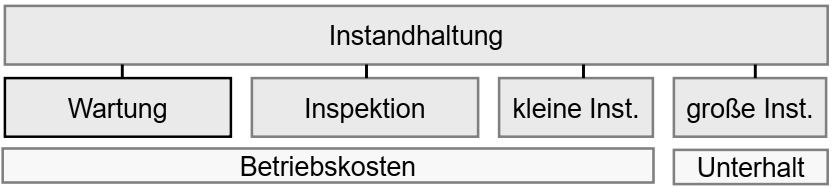
\includegraphics[width=0.45\textwidth]{Grafiken/Instandhaltung/GEFMA 122 Instandhaltung.png}
                    \item Kleine Instandsetzung:\\
                        Austausch von Verschleißteilen. Diese Leistung wird in der Praxis vom Betriebs-personal oder im Zuge der Wartung ausgeführt.
                    \item Große Instandsetzung:\\
                        Jede Wiederherstellung des Sollzustandes, die über die kleine Instandsetzung hinausgeht. Früher als Reparatur bezeichnet.
                    \item Instandhaltungsziele:\\
                        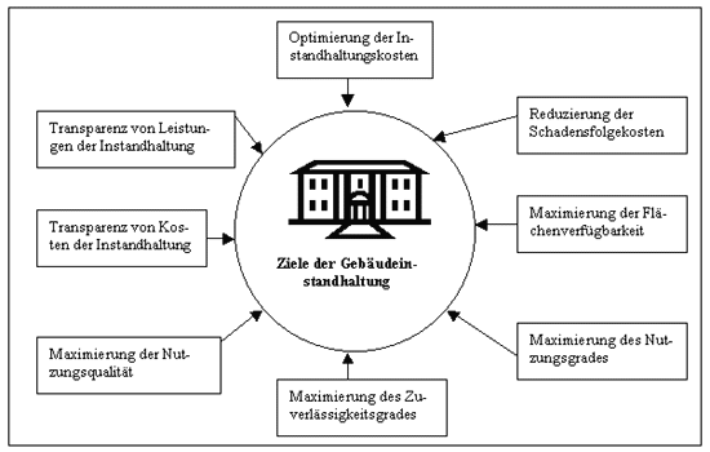
\includegraphics[width=0.45\textwidth]{Grafiken/Instandhaltung/Instandhaltungsziele.png}\\        
                \end{itemize}
        \end{itemize}


    \subsection{Instandhaltungsstrategien und deren Anwendungsbereiche}
        \begin{itemize}
            \item Strategie
                \begin{itemize}
                    \item Eine Strategie beschreibt eine Art und Weise, wie man seine Kräfte einsetzt.
                    \item Zum strategischen Denken und Handeln gehört das Ziel, das erreicht werden soll.
                \end{itemize}
            \item Umsetzung von Unternehmenszielen:\\
                Ziele $\rightarrow$ Strategie $\rightarrow$ Taktik $\rightarrow$ Operatives Geschäft\\
                Instandhaltungsziele müssen mit den Unternehmenszielen abgestimmt werden.
            \item Typische Unternehmensziele
                \begin{itemize}
                    \item Produktionssicherheit
                    \item hohe Verfügbarkeit der Anlagen 
                    \item Wirtschaftlichkeit und Minimierung des Kapitalbedarfs zur Erreichung eines positiven Betriebsergebnisses
                    \item Substanzerhaltung
                    \item Außenwirkung, die speziell im Bezug auf Gebäude eine Rolle spielt
                \end{itemize}
            \item Formulierung von Zielen (betriebswirtschaftliche Ziele)
                \begin{itemize}
                    \item Minimierung des Instandhaltungsaufwandes
                        \begin{itemize}
                            \item während der Nutzungszeit
                            \item bei definiertem Nutzungszweck
                        \end{itemize}
                    \item Optimierung der Kosten der Instandhaltung
                    \item Maximierung des Gewinnbeitrages
                    \item Einhaltung eines Instandhaltungsbudgets
                    \item Maximierung der Wirtschaftlichkeit
                    \item Minimierung des Kapitalbedarfs zur Erreichung eines positiven Betriebsergebnisses
                \end{itemize}
            \item Formulierung von Zielen (produktionstechn., ästhetische, gesetzliche und sicherheitstechn. Aspekte)
                \begin{itemize}
                    \item Erfüllung sicherheitstechnischer, durch Gesetze und Bestimmungen vorgegebener Anforderungen
                    \item Maximierung der Zuverlässigkeit
                    \item Erhöhung der Anlagenverfügbarkeit
                    \item Maximierung des Nutzungsgrades
                    \item Senkung der Störungsrate
                    \item Substanzerhaltung
                    \item Außenwirkung, z.B. durch eine Fassadenerneuerung an einem Gebäude
                \end{itemize}
            \item Präventive und Korrektive Instandhaltungsstrategien \label{Instandhaltungsstrategien}\\
                        \begin{minipage}{0.45\textwidth}
                            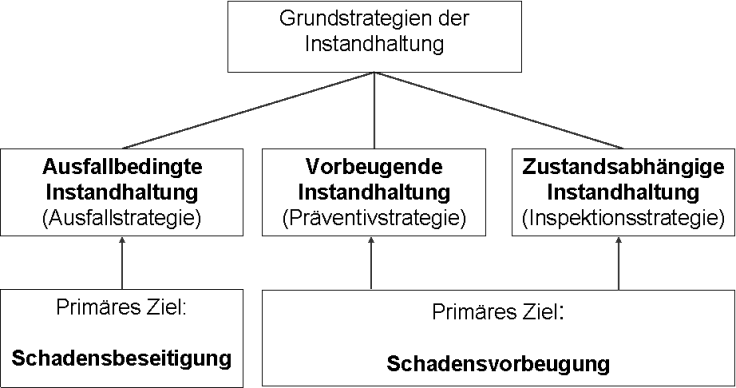
\includegraphics[width=0.99\textwidth]{Grafiken/Instandhaltung/Grundstrategien der Instandhaltung.png}
                        \end{minipage}
                        \begin{minipage}{0.5\textwidth}
                            \begin{itemize}
                                \item Ausfallbedingte Instandhaltung: Nicht möglich, wenn keine Ersatzflächen zur Verfügung steht z.B. Glühbirne wechseln\\
                                \item Zustandsabhängige Instandhaltung: Schaden auf keinen Fall eintreten lassen z.B. Inspektion Auto
                            \end{itemize}
                        \end{minipage}
            \item Präventivstrategie    
                \begin{itemize}
                    \item aktive Instandhaltung (Handeln bereits vor Schaden)
                    \item Bauteilversagen wird verhindert
                    \item Bauteilersatz nach einer festgelegten Betriebszeit
                    \item Abnutzungsvorrat wird nicht ausgenutzt
                \end{itemize}
                Auswirkung auf Lebensdauer:\\
                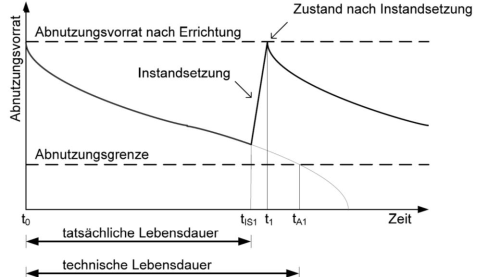
\includegraphics[width=0.55\textwidth]{Grafiken/Instandhaltung/Praeventivstrategie.png}\\
                Erkenntniss aus Gruppenarbeit:\\
                Instandsetzung erfolgt bei Überschreitung eines strategie vorher definierten Zeitpunktes.
                Voraussetzung:
                    \begin{itemize}
                        \item Genaue Kenntnis über den Ausfallzeitpunkt eines Bauteils.
                    \end{itemize}
                Problem:
                    \begin{itemize}
                        \item Ausfallzeitpunkt in Praxis nur schwer bestimmbar. Erfahrung im Betreiben des Elements muss vorhanden sein.
                    \end{itemize}
                Eine Vorbeugungsstrategie ist nur dann sinnvoll, wenn der erwartete Folgeschaden größer als der Restnutzen des Elementes ist!
            \item Inspektionsstrategie
                \begin{itemize}
                    \item Bauteilzustand wird durch Inspektionen genau bestimmt
                    \item Erneuerung bei Übersteigung einer vorher festgelegten Grenze
                    \item Ausfallschäden werden minimiert
                    \item Abnutzungsvorrat wird optimal ausgenutzt
                \end{itemize}
                Auswirkung auf Lebensdauer:\\
                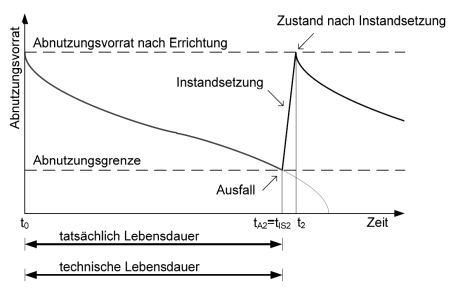
\includegraphics[width=0.55\textwidth]{Grafiken/Instandhaltung/Inspektionsstrategie.png}\\
                Erkenntniss aus Gruppenarbeit:
                \begin{itemize}
                    \item Abnutzungsvorrat der Elemente wird durch Inspektionen bestimmt. Erneuerung des Bauteils erfolgt, wenn Vorrat unter ein bestimmtes Sollmaß sinkt.
                \end{itemize}
                Voraussetzung:
                    \begin{itemize}
                        \item Inspektionen erfolgen in regelmäßigen Abständen. Hierdurch kann der Zeitpunkt für bestimmte Wartungs-, Inspektions- und Instandsetzungsarbeiten festgelegt werden.
                    \end{itemize}
                Durch die gute Planbarkeit der Maßnahmen und eine möglichen, optimalen Ausnutzung der technischen Lebensdauer, wird sie zur kostenoptimalen und flexiblen Instandhaltungsstrategie.
            \item Ausfallstrategie
                \begin{itemize}
                    \item Reaktive Instandhaltung (Handeln erst bei Schaden)
                    \item Risiko eines Bauteilversagens wird in Kauf genommen
                    \item Keine Wartungs- und Inspektionsmaßnahmen
                    \item Abnutzungsvorrat wird maximal ausgenutzt
                \end{itemize}
                Auswirkung auf Lebensdauer:\\
                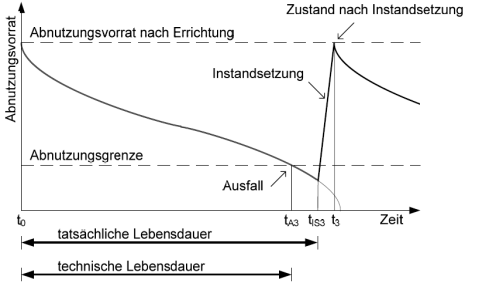
\includegraphics[width=0.55\textwidth]{Grafiken/Instandhaltung/Ausfallstrategie.png}\\
                Erkenntniss aus Gruppenarbeit:
                    \begin{itemize}
                        \item Instandsetzung erfolgt erst nach Eintritt eines Schadens
                    \end{itemize}
                Voraussetzung:
                    \begin{itemize}
                        \item Hohe Verfügbarkeit von Instandsetzungspersonal, um die Schäden schnell zu beheben, und somit einen langen Produktionsstillstand mit hohen Folgekosten zu vermeiden.
                    \end{itemize}
                Der Vorteil dieser Strategie ergibt sich durch eine optimale Ausnutzung der technischen Lebensdauer von Bauteilen. Kosten lassen sich nur scheinbar einsparen, da diese durch entstehende Folgekosten meist in kürzester Zeit egalisiert werden.
        \end{itemize}
\newpage


    
\section{Lebensdauer und Abnutzung von Bauteilen} \label{Nutzungs/Lebensdauer}

    \subsection{Einführung / Grundlagen}
        \begin{itemize}
            \item Lebensdauer bestimmt Anzahl der Austauschzyklen\\
                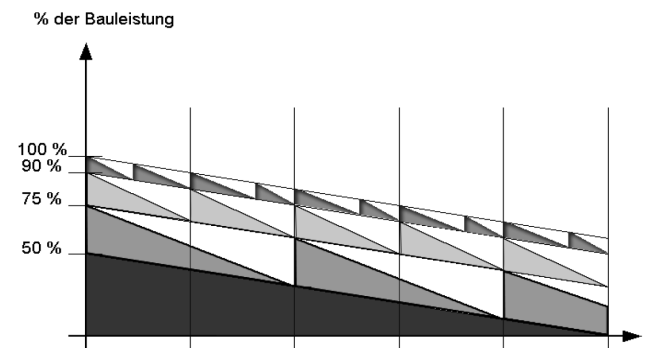
\includegraphics[width=0.55\textwidth]{Grafiken/Lebensdauer und Abnutzung von Bauteilen/Lebensdauer Austauschzyklen.png}
            \item Lebensdauerangaben
                \begin{itemize}
                    \item Lebenszykluskostenberechnungen (LCC)
                    \item Ökobilanzierungen (LCA)
                    \item Instandhaltungsplanung
                    \item Entscheidungshilfe bei der Auswahl von Bauteilen (Dauerhaftigkeit!)
                    \item Neubau
                    \item Umbau / Instandsetzung
                \end{itemize}
                $\Rightarrow$ Schlüsselrolle für:
                    \begin{itemize}
                        \item Lebenszyklusanalysen
                        \item Nachhaltigkeitszertifizierung
                        \item Integrale Planung
                    \end{itemize}
            \item Integrale Planung\\
                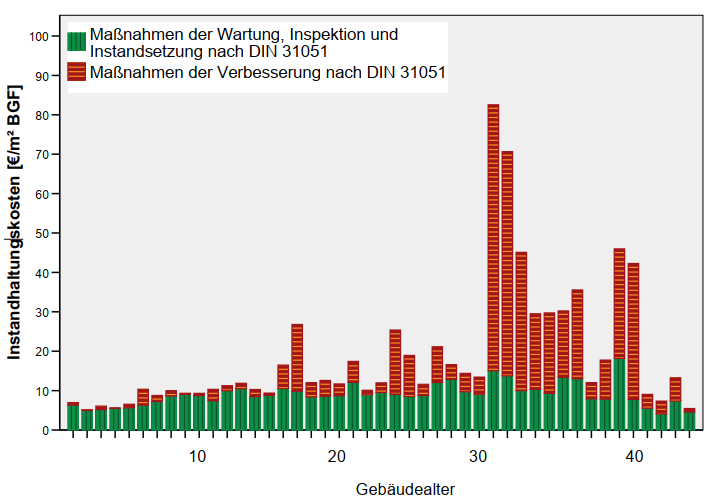
\includegraphics[width=0.55\textwidth]{Grafiken/Lebensdauer und Abnutzung von Bauteilen/Integrale Planung.png}
            \item Instandhaltungsstrategien / Instandhaltungsbudgetierung \\
                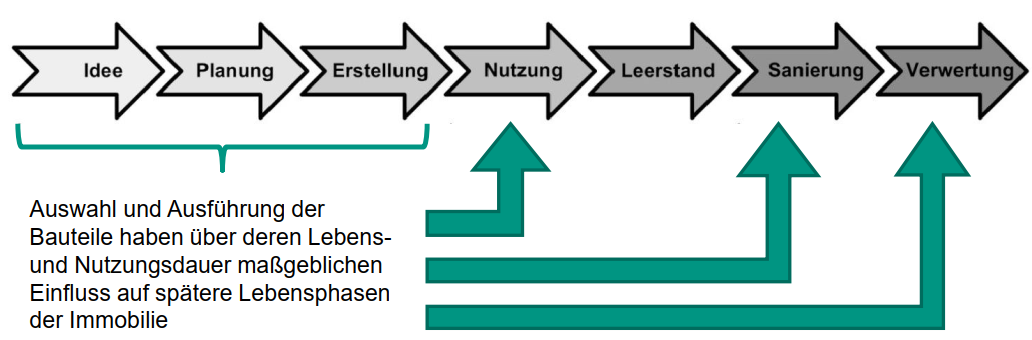
\includegraphics[width=0.55\textwidth]{Grafiken/Lebensdauer und Abnutzung von Bauteilen/Instandhaltungsstrategien ; Instandhaltungsbudgetierung.png}
            \item Arten der Lebensdauer
                \begin{itemize}
                    \item Technische Lebens- / Nutzungsdauer
                    \item Wirtschaftliche Lebens- / Nutzungsdauer
                \end{itemize}
        \subsection{Definitionen}
            \item Definition Lebensdauer:\\
                Die Lebensdauer ist definiert als Zeitdauer vom Beanspruchungsbeginn bis zum Zeitpunkt des Ausfalls eines einzelnen Bauelements oder eines zusammengesetzten, nicht mehr reparierbaren Systems
            \item Definition Nutzungsdauer:\\
                Die Nutzungsdauer ist jedoch als der Zeitraum definiert in dem ein Wirtschaftsgut des abnutzbaren Anlagevermögens betrieblich genutzt wird $\rightarrow$ Die Nutzungsdauer kann die Lebensdauer nie überschreiten
            \item Lebensdauer / Nutzungsdauer:
                \begin{itemize}
                    \item Beide Begriffe werden auch in der Fachwelt häufig synonym verwendet.
                    \item Dies betrifft insbesondere die technische Nutzungsdauer und die technische Lebensdauer
                    \item Bei Betrachtungen der Wirtschaftlichkeit steht der Begriff der Nutzungsdauer im Vordergrund, da die ökonomische Vorteilhaftigkeit aus
                    der Nutzbarmachung der Sache generiert wird
                \end{itemize}  
            \item Nutzungsdauer - Differenzierung \label{Nutzungsdauertypen}
                \begin{itemize}
                    \item Verwendungsdauer eines Anlagegutes differenziert in:
                        \begin{itemize}
                            \item Wirtschaftliche Nutzungsdauer (Zeitraum der rentablen Nutzung)
                            \item Technische Nutzungsdauer (Zeitraum bis zum körperlichen Verschleiß)
                            \item Rechtliche Nutzungsdauer (Zeitraum, in dem das Wirtschaftsgut genutzt werden darf).
                            \item Mit der Nutzungszeit steigende Instandhaltungskosten und technischer Fortschritt führen i.d.R. zu einer starken Divergenz zwischen technischer Nutzungsdauer und wirtschaftlicher Nutzungsdauer.
                        \end{itemize}
                \end{itemize}
            \item Technische / Funktionelle Nutzungsdauer
                \begin{itemize}
                    \item Die technische Nutzungsdauer einer Komponente oder eines Bauteils kann beschrieben werden als Zeitraum, in dem diese „physisch zur Verfügung steht und den geforderten Eigenschaften ohne Einschränkungen entspricht
                \end{itemize}
                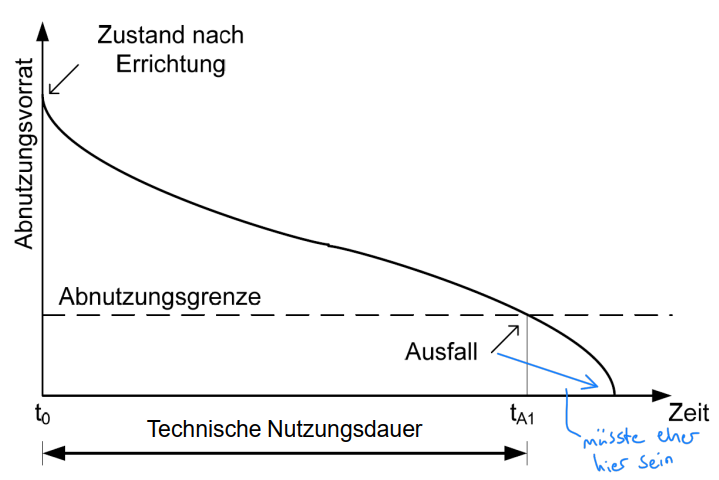
\includegraphics[width=0.55\textwidth]{Grafiken/Lebensdauer und Abnutzung von Bauteilen/Technische - Funktionelle Nutzungsdauer.png}
                \begin{itemize}
                    \item Maximale Nutzbarkeit
                    \item Zeitspanne in der Bauteil seine Funktion erfüllt
                    \item Zeitraum zwischen Einbau und Ausfall
                    \item Ende der technischen Nutzungsdauer ist erreicht, wenn
                        \begin{itemize}
                            \item Abnutzungsvorrat aufgebraucht ist
                            \item Instandhaltung nicht mehr möglich ist
                        \end{itemize}
                \end{itemize}
                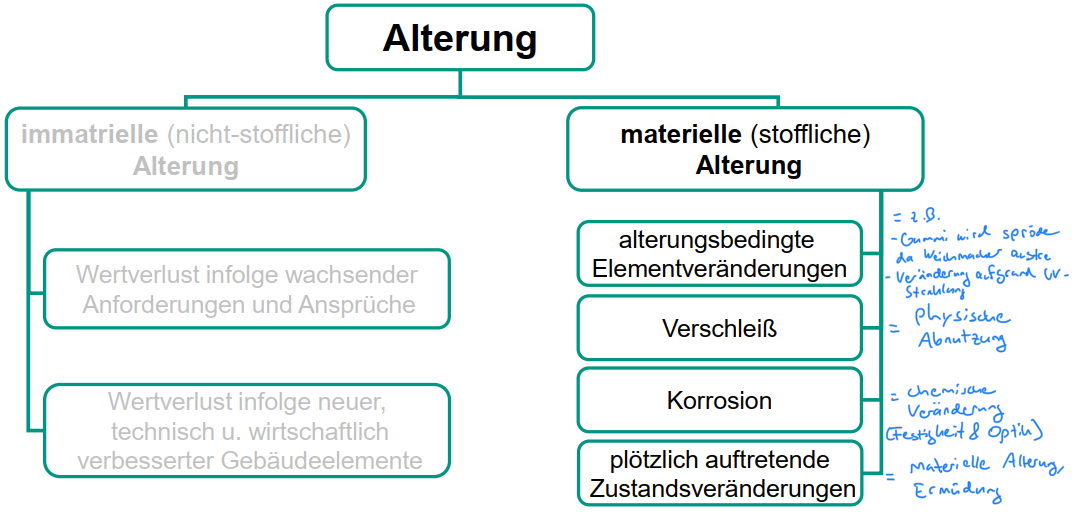
\includegraphics[width=0.55\textwidth]{Grafiken/Lebensdauer und Abnutzung von Bauteilen/Alterung.png}
            \item Wirtschaftliche Nutzungsdauer
                \begin{itemize}
                    \item Zeitspanne in der Nutzung wirtschaftlich sinnvoll ist
                    \item Ende der wirtschaftlichen Lebens- / Nutzungsdauer ist erreicht, wenn
                        \begin{itemize}
                            \item Kosten die Erträge übersteigen
                            \item Alternativen höhere Renditen erwirtschaften
                        \end{itemize}
                    \item Ist i.d.R. kürzer als technische Nutzungsdauer
                \end{itemize}
                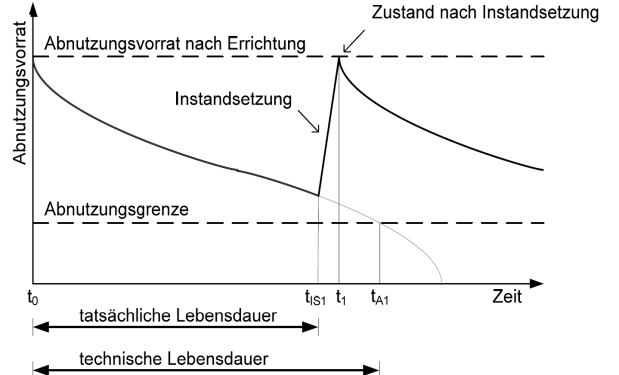
\includegraphics[width=0.45\textwidth]{Grafiken/Lebensdauer und Abnutzung von Bauteilen/Wirtschaftliche Nutzungsdauer.png}
                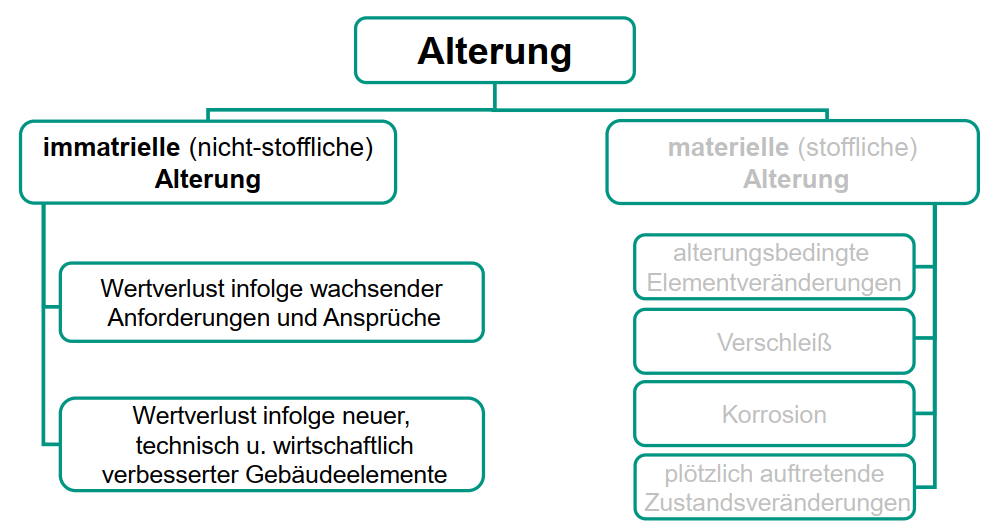
\includegraphics[width=0.45\textwidth]{Grafiken/Lebensdauer und Abnutzung von Bauteilen/Wirtschaftliche Alterung.png}
            \item Betriebsgewöhnliche Nutzungsdauer:\\
                Zeitraum, in dem ein Wirtschaftsgut voraussichtlich seiner Zweckbestimmung nach benutzt werden kann; bei gebraucht angeschafften Wirtschaftsgütern die voraussichtliche Restnutzungsdauer. Die betriebsgewöhnliche Nutzungsdauer ist unter Berücksichtigung der bes. Verhältnisse zu schätzen. In der Kostenrechnung bestimmt die betriebsgewöhnliche Nutzungsdauer direkt den Abschreibungszeitraum.
            \item Tatsächliche Betriebsdauer
                \begin{itemize}
                    \item Die technische Nutzungsdauer einer Bohrmaschine im Privathaushalt beträgt in der Regel mehrere Jahrzehnte.
                    \item Die tatsächliche durchschnittliche Betriebsdauer einer Bohrmaschine beträgt im Schnitt ca. 13 Minuten
                \end{itemize}

        \subsection{Lebensdauern als Basisinformation zur Erarbeitung von Instandhaltungsstrategien}
            \item Instandhaltungsstrategie: Ermittlung des Optimums bezüglich Art- und Zeitpunkt der Maßnahmen
            \begin{minipage}{0.5\textwidth}
            \item Mögliche Strategie für das Bauteil Dach\\
                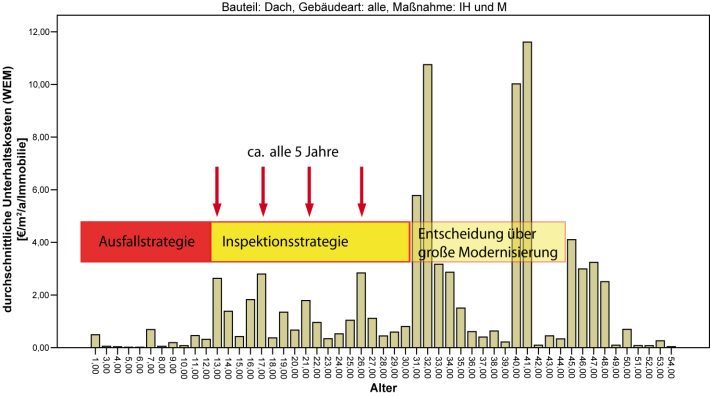
\includegraphics[width=0.85\textwidth]{Grafiken/Lebensdauer und Abnutzung von Bauteilen/Strategie Dach.png}
            \end{minipage}
            \begin{minipage}{0.5\textwidth}
            \item Mögliche Strategie für Elektroinstallationen\\
                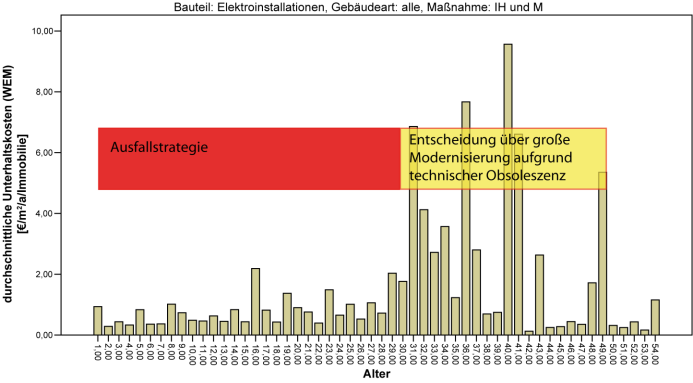
\includegraphics[width=0.85\textwidth]{Grafiken/Lebensdauer und Abnutzung von Bauteilen/Strategie Elektro.png}
            \end{minipage}
            
        \subsection{Obsoleszenzen} \label{Obsoleszenzen}
                \begin{itemize}
                    \item \textbf{Funktionale Obsoleszenz:}\\
                    Die Funktion eines Gebäudes oder dessen Teilsysteme entspricht nicht
                    mehr den Anforderungen
                    \item \textbf{Technische Obsoleszenz:}\\
                    Ein Gebäude oder dessen Teilsysteme entsprechen nicht mehr aktuellen
                    technischen Standards bzw. den gestiegenen Anforderungen. Besonders maßgebend im TGA-Bereich
                    \item \textbf{Materielle Obsoleszenz:}\\
                    Bezeichnet die eigentliche physische Alterung des Gebäudes bzw. seiner
                    Teile
                    \item \textbf{Ökonomische Obsoleszenz:}\\
                    Tritt ein, wenn ein Gebäude oder dessen Teilsysteme nicht mehr rentabel
                    betrieben werden kann
                    \item \textbf{Rechtliche Obsoleszenz:}\\
                    Ein Gebäude oder dessen Teilsysteme kann nicht mehr mit vernünftigem
                    Aufwand an die bestehende Gesetze oder Vorschriften angepasst werden. Siehe EnEV-Vorschriften bzw. GEG
                    \item \textbf{Formale Obsoleszenz:}\\
                    Bezieht sich auf die formalen Kriterien, sie ist deshalb am stärksten durch
                    subjektive Maßstäbe bestimmt. Bauten entsprechen nicht mehr dem
                    „Geschmack“ der Zeit. Siehe Wandel kleine Einzelzimmer zu größeren offenen Raumkonzept
                    \item \textbf{Geplante Obsoleszenz:}\\
                    Gezielt geplant und herbeigeführter Ausfall eines Gebäude oder technischen
                    Einheit mit dem Ziel die technische Nutzungsdauer systematisch zu verkürzen. Technik in TGA nur auf Gewährleistungszeitraum ausgelegt.
                \end{itemize}
        \subsection{Materielle Alterung} \label{EinflussBauteile}
                \begin{itemize}
                    \item Luftverschmutzung (Schwefeldioxid, Stickoxide, Ozon, Aerosole)\\
                        Schwefeldioxid verwandelt Kalk (CaCO3) in Gips (CaSO4). Gips ist wasserlöslicher als Kalk und poröser:
                            \begin{itemize}
                                \item Auswaschungen durch Regen $\rightarrow$ Substanzverlust
                                \item Verstärkte Absorption von Wasser $\rightarrow$ Frostschäden
                                \item Verstärkte Absorption von Partikeln $\rightarrow$ Verfärbungen (z.B. Russpartikel durch Autoabgase) (Schwärzungen)
                            \end{itemize}
                    \item Feuchtigkeit (Frost-Tau-Wechsel)
                    \item Unsachgemäße Restaurierungsmaßnahmen
                        \begin{itemize}
                            \item Einsatz von Zementmörtel zur Restaurierung:\\
                                In der Mittelalterlichen Stadt von Rhodos wurde Zementmörtel bei der Restaurierung des Mauerwerks verwendet. Da die mechanischen Eigenschaften und die Mikrostruktur des neuen Mörtels sich vom vorhandenen Material unterscheiden, verstärkte diese Maßnahme die Abwitterung der eingeschlossenen originalen Mauersteine (Porensteine).
                            \item Einsatz von Metallverbindungen:\\
                                Unter Bewitterung oxidiert das Metall, das als Verbindung zwischen zwei Marmorblocken eingesetzt wurde. Durch den Oxidationsprozess vergrößert sich das Volumen des Metalls beträchtlich. Dies führt zu großem mechanischem Druck, der zum Versagen (Bruch) des umgebenden Materials führt, wenn er dessen Druckfestigkeit übersteigt.
                        \end{itemize}
                \end{itemize}    
        \end{itemize}

    \subsection{Einfluss der Instandhaltung auf die Lebensdauer von Bauteilen}
        \begin{itemize}
            \item Einfluss der Instandhaltung\\
                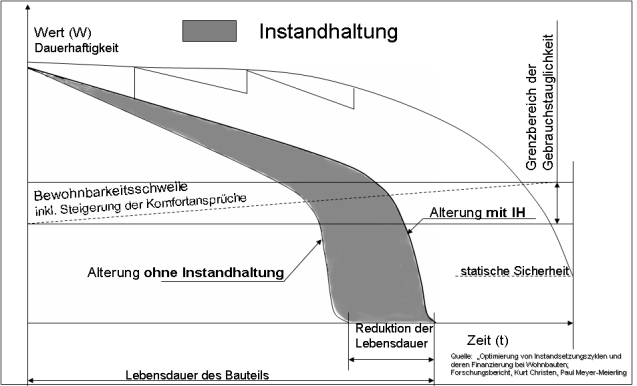
\includegraphics[width=0.45\textwidth]{Grafiken/Lebensdauer und Abnutzung von Bauteilen/Einfluss Instandhaltung.png}
            \item Einfluss der Instandhaltungsqualität\\
                    \begin{minipage}{0.4\textwidth}
                        Holzfenster $60 \%$ IH-Qualität, Lebensdauer auf $ L_{I H}=L \cdot\left(1-r_{I H} \cdot\left(1-IH_{\text {Qual }}\right)\right) $ von 45 auf 36 Jahre reduziert.\\
                        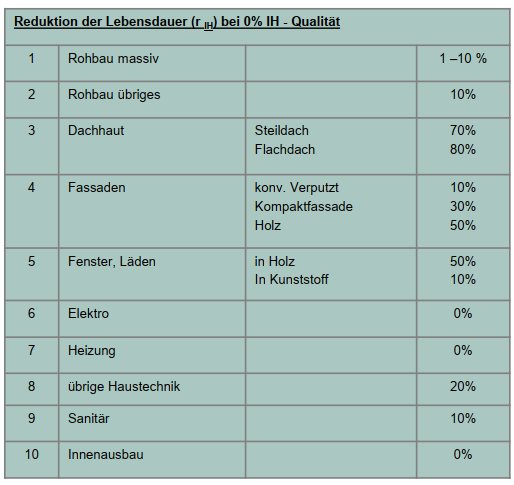
\includegraphics[width=0.99\textwidth]{Grafiken/Lebensdauer und Abnutzung von Bauteilen/Einfluss IH Qualitaet.png}
                    \end{minipage}\hspace{2mm}
                    \begin{minipage}{0.52\textwidth} 
                        Einfluss der Instandhaltungsqualität auf die Lebensdauern verschiedener Gebäudeelemente\\
                        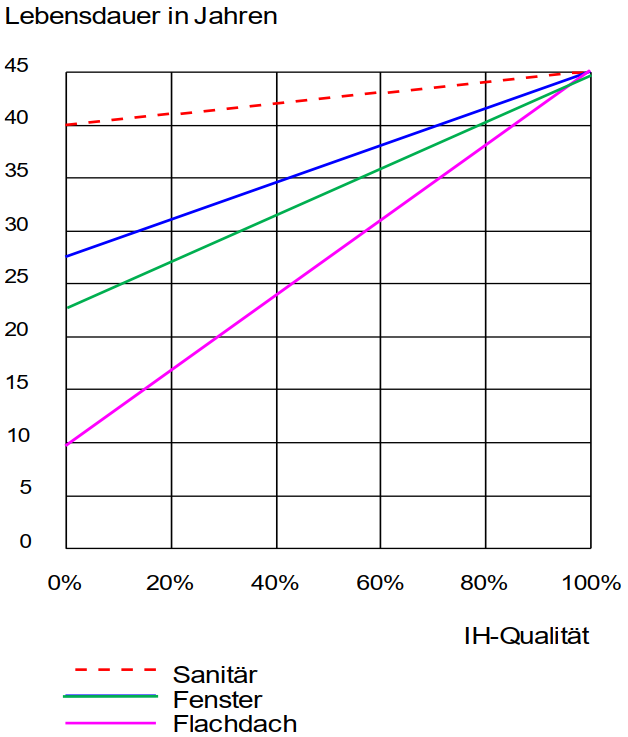
\includegraphics[width=0.65\textwidth]{Grafiken/Lebensdauer und Abnutzung von Bauteilen/Einfluss IH Qualitaet 2.png}
                    \end{minipage}\\ \vspace{2mm}
                    $\Rightarrow$ Hohe IH-Qualität sorgt für lange Lebensdauer
        \end{itemize}
    \subsection{Verständnisfragen zu Themenabschnitt}
        \begin{itemize}
            \item Wann ist das Ende der wirtschaftlichen Nutzungsdauer erreicht?
                \begin{itemize}
                    \item Wenn die Kosten die Erträge übersteigen
                    \item Wenn Alternativen höhere Renditen erwirtschaften
                \end{itemize}
            \item Welche Obsoleszenz bezeichnet die eigentliche physische Alterung des Gebäudes bzw. seiner Teile?
                \begin{itemize}
                    \item Die Materielle Obsoleszenz
                \end{itemize}
            \item Nennen Sie drei typische materielle (stoffliche) Alterungsarten
                \begin{itemize}
                    \item altersbedingte Elementveränderung
                    \item Verschleiß
                    \item Korrosion
                    \item Plötzlich auftretende Zustandsveränderung
                \end{itemize}
        \end{itemize}

\newpage

\section{Bestimmung von Bauteillebensdauern} \label{BTLD}
    
    \subsection{Verfahren zur Bestimmung Bauteillebensdauern / techn. Nutzungsdauern}
        Methoden zur Bestimmung von Bauteillebensdauern:
        \begin{itemize}
            \item Kennwerte (Beispiel aus Publikationen)
                \begin{itemize}
                    \item Meist Angabe von Spannen (min, max) oder mittlere Lebensdauer
                    \item Starke Abweichung der Lebensdauerangaben
                    \item Unterschiedliche Quellen
                        \begin{itemize}
                            \item Herstellerangaben (Garantiezeiten, oder marktstrategische Gründe)
                            \item Forschungsergebnisse
                            \item Erfahrungswerte
                        \end{itemize}
                    \item Randbedingungen sind nicht dokumentiert.
                    \item Keine standardisierte Ermittlung von Kennwerten
                    \item Es gibt kein „richtig“ oder „falsch“, da Einflüsse unterschiedlich
                    $\Rightarrow$ Einflussfaktoren wie z.B. Lage des Bauteils, Klima, Nutzung usw. spielen eine wichtige Rolle!\\
                    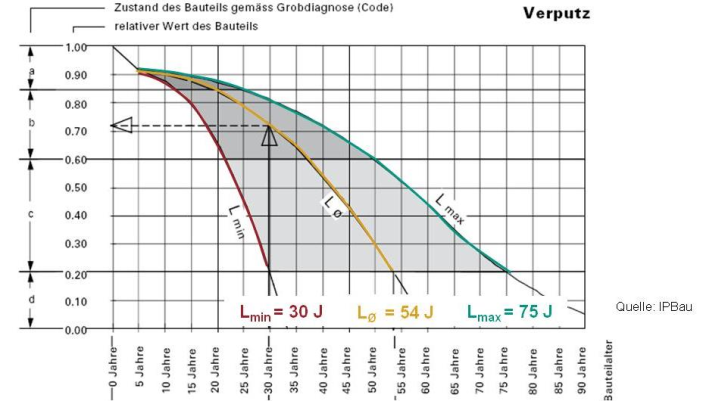
\includegraphics[width=0.5\textwidth]{Grafiken/Verfahren zur Bestimmung von Bauteillebensdauern/Einfluss Umweltbedingungen.png}
                \end{itemize}
            \item Referenzfaktorenmethode von Tomm, Rentmeister und Finke
                \begin{itemize}
                    \item \enquote{Verfahren zur systematischen Erfassung und Steuerung von Instandhaltungsmaßnahmen an Gebäuden}
                    \item Maßnahmenintervallplan für 100 verschiedene Bauteile:\\
                        \resizebox{0.85\textwidth}{!}{\begin{tabular}{|l|l|} \hline
                                Basis: & mittlere Lebensdauer\\
                                Einflussfaktoren: & Nutzung, Umwelteinflüsse, Bauteilqualität, Instandhaltungsintensität \\
                                Abzugsfaktoren: & Elementalter oder Abnutzung \\ \hline
                                Resultat: & Restlebensdauer \\ \hline
                        \end{tabular}}\\
                        \resizebox{0.86\textwidth}{!}{\begin{tabular}{l r}
                              \phantom{I sometimes hate LaTex and my utter incompetence ;)} & \tiny (LBB und ARGEBAU), 1995
                        \end{tabular}}
                    \item Basis bildet mittlere Lebensdauererwartung (Anhand eines Bauelementekataloges, in dem die instandhaltungsrelevanten Bauteile gemäß DIN 276 gegliedert werden. Die Angaben zu den mittleren Lebensdauern basieren auf Daten und Erkenntnissen aus der Literatur, eigenen Erfahrungen der Bearbeiter sowie Informationen von externen Fachleuten und Firmeninformationen.)
                    \item Subjektive Einschätzung der Abzugsfaktoren (Es wird keine Rechenvorschrift und auch keine Gewichtung der Einflüsse vorgegeben!\\ $\rightarrow$ Verkürzung oder die Verlängerung der Lebensdauer muss durch den Anwender anhand seiner individuellen Erfahrung den spezifischen Verhältnissen entsprechend erfolgen.)
                    \item Lineare Vereinfachung des Abnutzungsverhaltens
                \end{itemize}
            \item Faktorenmethode der ISO 15686 \label{ISO15686}
                \begin{itemize}
                    \item Basiert auf der Annahme, dass die Lebensdauer eines Bauteils maßgeblich durch Einflüsse auf die Bauteilqualität, durch Umgebungseinflüsse und Nutzungsbedingungen geprägt wird.
                    \item Die ISO 15686 definiert sieben Einflussfaktoren (A bis G), die bei der Ermittlung der zu erwartenden Bauteillebensdauer zu berücksichtigen sind.
                    \item $ESCL= RSCL\cdot Faktor A \cdot FaktorB \cdot FaktorC \cdot FaktorD \cdot FaktorE \cdot FaktorF \cdot FaktorG$
                        \begin{itemize}
                            \item $ESCL$: Spezifische Bauteillebensdauer (estimated service life)
                            \item $RSCL$: Referenzlebensdauer (reference service life)
                        \end{itemize}
                    \item Einflussgrößen:\\
                        \resizebox{0.85\textwidth}{!}{$\begin{array}{lcll}
                            \hline \text { Qualität } & \text { A } & \text { Bauteilqualität } & \begin{array}{l}
                            \text { Herstellung, Lagerung, Transport, } \\
                            \text { Materialien, Schutzschicht }
                            \end{array} \\
                            \hline & \text { B } & \text { Konstruktionsqualität } & \text { Eingliederung, konstruktiver Schutz } \\
                            \cline { 2 - 4 } & \text { C } & \text { Ausführungsqualität } & \begin{array}{l}
                            \text { Einbau auf der Bautstelle, klimatische } \\
                            \text { Bedingungen auf der Baustelle }
                            \end{array} \\
                            \hline \text { Umgebung } & \text { D } & \text { innerhalb des Gebäudes } & \text { Raumluftbedingungen, Kondensation } \\
                            \cline { 2 - 4 } & \mathrm{E} & \text { ausserhalb des Gebäudes } & \begin{array}{l}
                            \text { Standort, Wetter, Luftverschmutzung, } \\
                            \text { Bauwerkserschütterungen }
                            \end{array} \\
                            \hline \text { Nutzungsbedingungen } & \mathrm{F} & \text { Nutzung } & \begin{array}{l}
                            \text { mechanische Einflüsse, Art der Nutzung, } \\
                            \text { Verschleiß }
                            \end{array} \\
                            \cline { 2 - 4 } & \text { G } & \text { Instandhaltungsqualität } & \begin{array}{l}
                            \text { Qualtiät und Zyklus der Instandhaltung, } \\
                            \text { Zugänglichkeit für Instandhaltung }
                            \end{array} \\
                            \hline
                            \end{array}$} \vspace*{3mm}
                    \item Analyse und Verbesserung der Faktorenmethode:\\
                        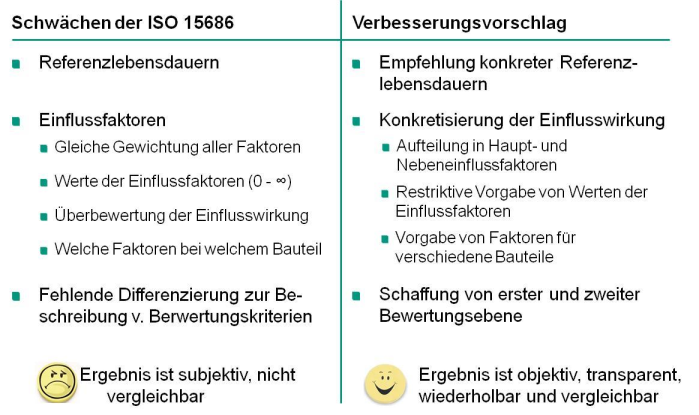
\includegraphics[width=0.55\textwidth]{Grafiken/Verfahren zur Bestimmung von Bauteillebensdauern/Analyse und Verbesserung der Faktorenmethode.png}
                    \item Einflussfaktoren: Wirkungsstärke:\\
                            Empfehlung nach ISO: Werte von 0,8 bis 1,2:\\
                        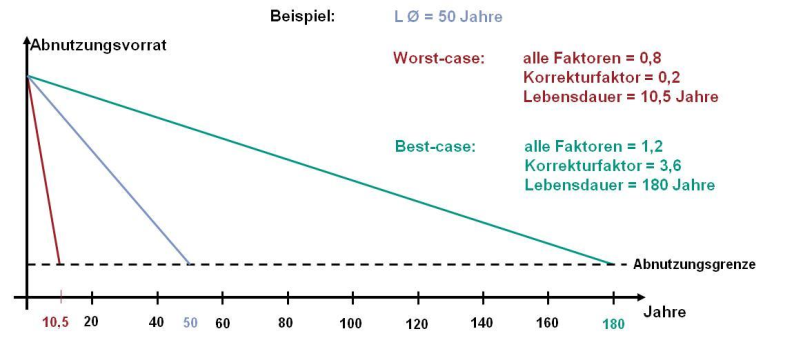
\includegraphics[width=0.65\textwidth]{Grafiken/Verfahren zur Bestimmung von Bauteillebensdauern/Einflussfaktoren - Wirkungsstaerke.png}
                    \item Einflussfaktoren: Gewichtung und Kategorien:
                        \begin{itemize}
                            \item Differenzierung nach Wichtigkeit bzw. Einflussstärke:
                                \begin{itemize}
                                    \item Haupteinflussfaktor
                                    \item Nebeneinflussfaktor
                                \end{itemize}
                            \item Beschränkung der Gewichtungsfaktoren:\\
                                \begin{tabular}{|l|c|c|c|}
                                \cline { 2 - 4 } \multicolumn{1}{c|}{} & $\begin{array}{c}\text { LD verkürzend } \\
                                -\end{array}$ & $\begin{array}{c}\text { durchschnittlich } \\
                                \varnothing\end{array}$ & $\begin{array}{c}\text { LD verlängernd } \\
                                +\end{array}$ \\
                                \hline Hauptfaktor & $\mathbf{0 , 8} / \mathbf{0 , 9}$ & $\mathbf{1 , 0}$ & $\mathbf{1,1}$ \\
                                \hline Nebenfaktor & $\mathbf{0 , 9} / \mathbf{0,95}$ & $\mathbf{1 , 0}$ & $\mathbf{1 , 0 5}$ \\
                                \hline
                                \end{tabular}
                            \item Pro Einflussfaktor 2 Ebenen an Gewichtungsfaktoren (1. sehr grob, 2. spezifischer)
                        \end{itemize}
                    \item Modellablauf in 4 Schritten:
                        \begin{itemize}
                            \item 1. Schritt: 
                                \begin{itemize}
                                    \item Ermittlung maßgeblicher Einflussfaktoren (Haupt- und Nebenfaktoren)
                                \end{itemize}
                            \item 2. Schritt: 
                                \begin{itemize}
                                    \item Bestimmung der Gewichtungsfaktoren
                                    \item Kategorien (- / Ø / +) werden durch vorgegebene Kriterien beschrieben
                                \end{itemize} 
                            \item 3. Schritt: 
                                \begin{itemize}
                                    \item Zuordnung in Kategorien
                                \end{itemize}
                            \item 4. Schritt: 
                                \begin{itemize}
                                    \item Bestimmung der rechnerischen Lebensdauer
                                    \item Rechnerische Lebensdauer $=$ Referenzlebensdauer $\cdot$ Korrekturfaktor\\
                                            Korrekturfaktor $=$ Faktor A1 $\cdot$ Faktor A2 $\cdot$ Faktor $\cdot _{\dots} \cdot$ Faktor G
                                \end{itemize}
                        \end{itemize}
                    \item Beispiel Alu-Fensterflügel:\\
                        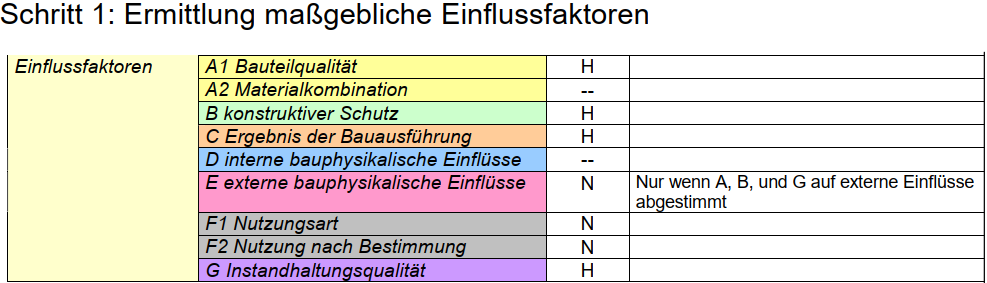
\includegraphics[width=0.45\textwidth]{Grafiken/Verfahren zur Bestimmung von Bauteillebensdauern/Alu-1.png}
                        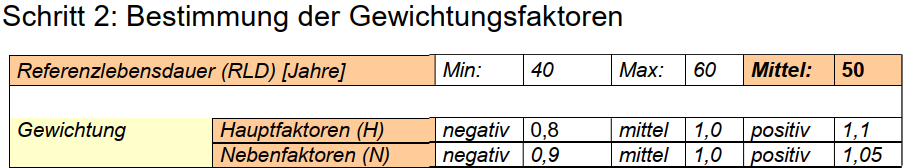
\includegraphics[width=0.45\textwidth]{Grafiken/Verfahren zur Bestimmung von Bauteillebensdauern/Alu-2.png}\\
                        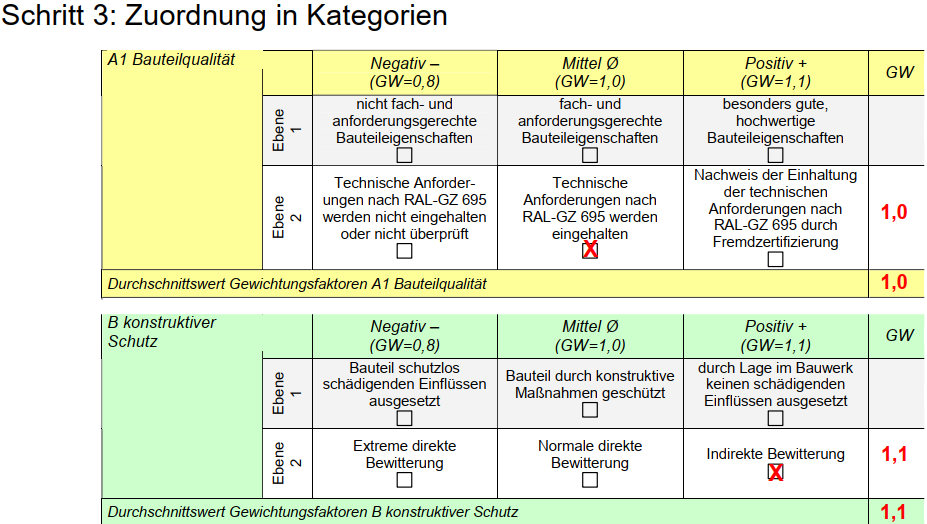
\includegraphics[width=0.4\textwidth]{Grafiken/Verfahren zur Bestimmung von Bauteillebensdauern/Alu-3.png}
                        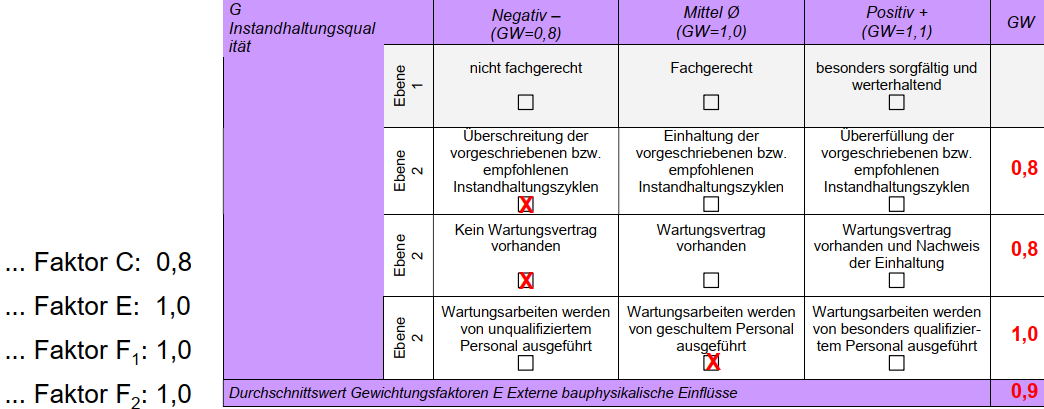
\includegraphics[width=0.5\textwidth]{Grafiken/Verfahren zur Bestimmung von Bauteillebensdauern/Alu-3.1.png}\\
                        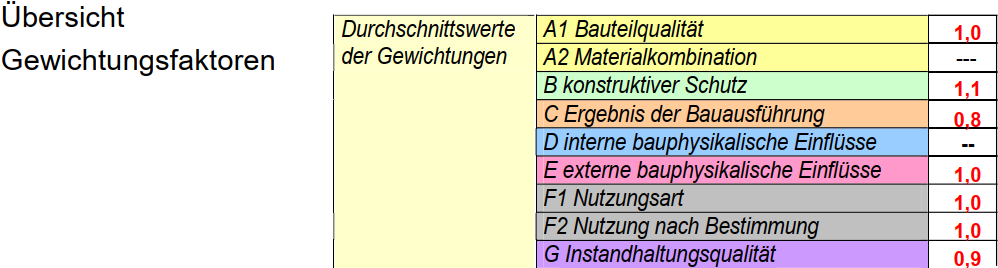
\includegraphics[width=0.45\textwidth]{Grafiken/Verfahren zur Bestimmung von Bauteillebensdauern/Alu-3.2.png}
                        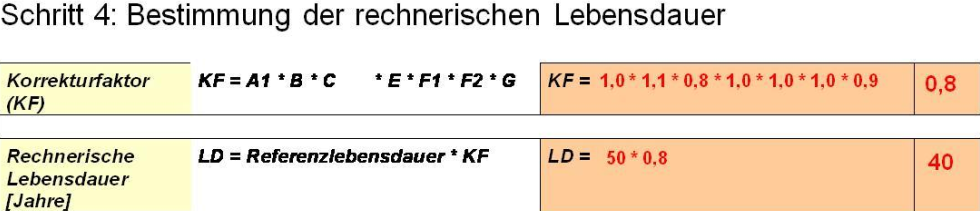
\includegraphics[width=0.45\textwidth]{Grafiken/Verfahren zur Bestimmung von Bauteillebensdauern/Alu-4.png}
                        \vspace*{3mm}
                        
                    \begin{minipage}{0.5\textwidth}
                            \item Schlussfolgerung: Ergebnis abhängig von...
                                \begin{itemize}
                                    \item Referenzlebensdauer
                                    \item Wahl der Faktoren
                                    \item Gewichtung der Faktoren
                                \end{itemize}
                            $\Rightarrow$ Enormes Fachwissen erforderlich!
                            \item  Durch Eingrenzung Entscheidungsspielraums wird Ergebnis objektiv, transparent, wiederholbar und vergleichbar.\\
                            Arbeitshilfen:
                                \begin{itemize}
                                    \item Bereitstellung von notwendigem Fachwissen
                                    \item Konkrete Vorgaben zu
                                        \begin{itemize}
                                            \item Kriterien und Grenzwerten
                                            \item Einflussfaktoren und Gewichtungen
                                        \end{itemize}
                                    \item In Form von Expertendatenblättern
                                \end{itemize}
                            \item Dadurch:
                                \begin{itemize}
                                    \item Ausschluss von verfälschender Wahl der Faktoren
                                    \item Eingrenzung des Entscheidungsspielraumes
                                    \item Erhöhung der Aussagekraft und Vergleichbarkeit
                                \end{itemize}
                        \end{minipage}
                    \begin{minipage}{0.5\textwidth}
                        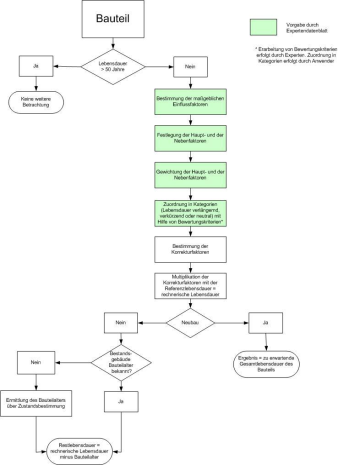
\includegraphics[width=0.8\textwidth]{Grafiken/Verfahren zur Bestimmung von Bauteillebensdauern/Entscheidungsfluss Restlebensdauer.png}
                    \end{minipage}
                \end{itemize}
        \end{itemize}

    \subsection{Abnutzungsmodelle}
        \begin{itemize}
            \item Kurven zeitabhängiger Abnutzung:\\
                \begin{minipage}{0.7\textwidth}
                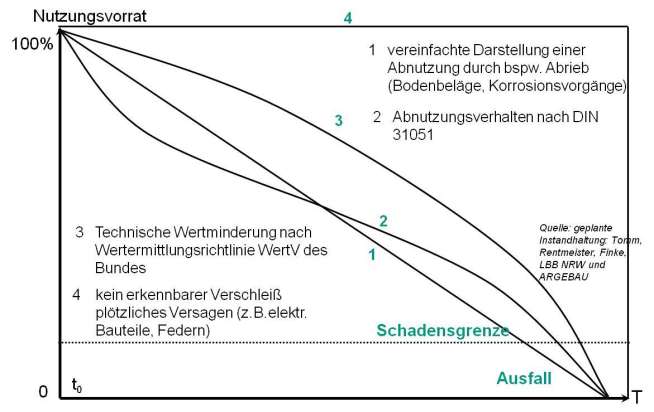
\includegraphics[width=0.99\textwidth]{Grafiken/Verfahren zur Bestimmung von Bauteillebensdauern/Kurven zeitabhaengiger Abnutzung.png}
                \end{minipage}
                \begin{minipage}{0.25\textwidth}
                1: Bremsen Auto, \\ Spundwand an Hafen $\dots$ \\ 3: dynamische Abnutzung
                \end{minipage}
            \item Wertverlust nach Schröder
                \begin{itemize}
                    \item Wertverlustkurven:\\
                        \begin{minipage}{0.4\textwidth}
                        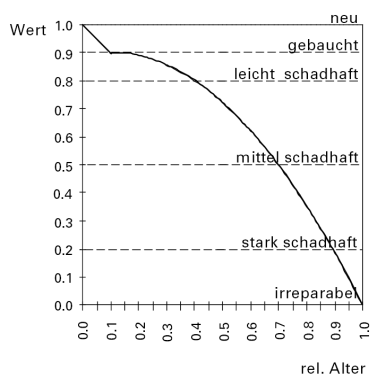
\includegraphics[width=0.7\textwidth]{Grafiken/Verfahren zur Bestimmung von Bauteillebensdauern/Wertverlustkurven - Wertverlust nach Schroeder.png}
                        \end{minipage}
                        \begin{minipage}{0.55\textwidth}
                            $W = 1-t^a$\\
                            $W$ = relativer Wert eines Bauteils\\
                            $t$ = relatives Alter eines Bauteils\\
                            $a$ = Exponent in der Entwertungsformel
                        \end{minipage}
                    \item Unterschiedliche Alterungsgeschwindigkeit:\\
                        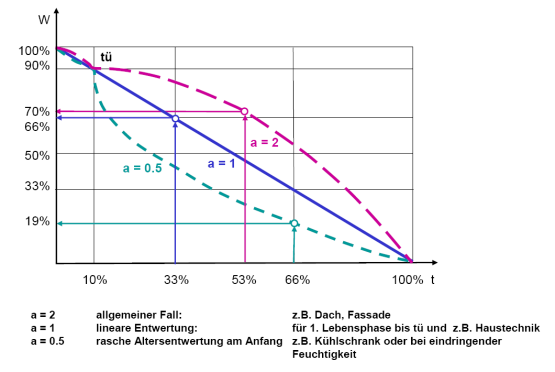
\includegraphics[width=0.65\textwidth]{Grafiken/Verfahren zur Bestimmung von Bauteillebensdauern/Wertverlustkurven - Wertverlust nach Schroeder untersch. Alt.GEschw..png}
                    \item Unterschiedliche Alterungsgeschwindigkeit:\\
                        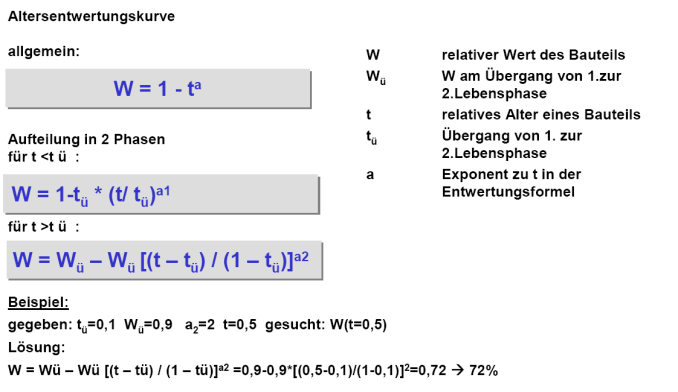
\includegraphics[width=0.65\textwidth]{Grafiken/Verfahren zur Bestimmung von Bauteillebensdauern/Wertverlustkurven - Wertverlust nach Schroeder allg. Formel.png}
                    \item Unterschiedliche Alterungsgeschwindigkeit:\\
                        \includegraphics[width=0.65\textwidth]{Grafiken/Verfahren zur Bestimmung von Bauteillebensdauern/Wertverlustkurven - Wertverlust nach Schroeder Bsp.png}\\ Übergangszeitpunkt (Knick) muss definiert sein
                \end{itemize}
            \item Wertverlust nach IPBau
                \begin{itemize}
                    \item Alterungsverhalten von Bauteilen und Unterhaltskosten: \\ Grundlagendaten für den Unterhalt und die Erneuerung von Wohnbauten\\
                    \begin{minipage}{0.5\textwidth}
                        \includegraphics[width=0.99\textwidth]{Grafiken/Verfahren zur Bestimmung von Bauteillebensdauern/IPBau 1.png}
                        \end{minipage}
                        \begin{minipage}{0.3\textwidth}
                            \item Erneuerungsdaten von \\120 Immobilien.
                            \item Entwicklung von \\Alterungskurven für 12 Bauteile.
                            \item Starke Streuung \\Alterungsverläufe wird deutlich.
                        \end{minipage}\\
                \end{itemize}
                    \includegraphics[width=0.75\textwidth]{Grafiken/Verfahren zur Bestimmung von Bauteillebensdauern/IPBau 2.png}\\
                    \includegraphics[width=0.75\textwidth]{Grafiken/Verfahren zur Bestimmung von Bauteillebensdauern/IPBau 3.png}\\
                    \includegraphics[width=0.75\textwidth]{Grafiken/Verfahren zur Bestimmung von Bauteillebensdauern/IPBau 4.png}
        \end{itemize}
    
    
    
    \subsection{Bauteilgruppen}
        \begin{itemize}
            \item Instandhaltung in der Praxis: Bauteilgruppen
                \begin{itemize}
                    \item Gebäude setzt sich aus Einzelbauteilen zusammen
                    \item Jedes Bauteil hat spezifisches Alterungsverhalten / Lebensdauer
                    \item Instandhaltung in der Praxis: Bildung von Bauteilgruppen
                \end{itemize}
            \item Gründe für Maßnahmenbündelung
                \begin{itemize}
                    \item Funktionelle Abhängigkeiten
                        \begin{itemize}
                            \item Bauteile werden bei Maßnahmen beschädigt oder zerstört
                            \item z.B. Erneuerung Außenputz erfordert neuen Anstrich
                        \end{itemize}
                    \item Logistische Zusammenhänge
                        \begin{itemize}
                            \item Baustelleneinrichtung kann gleichzeitig für mehrere Maßnahmen genutzt werden
                            \item Stehendes Gerüst kann optimal ausgenutzt werden\\
                               $\rightarrow$ Logistik/Infrastruhtur schon da oder Sperrpanse wegen anderer Arbeiten
                        \end{itemize}
                    \item Reduktion der Nutzerbeeinträchtigung
                        \begin{itemize}
                            \item z.B. durch Lärm oder Schmutz\\
                                $\rightarrow$ Bauteile in Baugruppen sollten sich in Zyklus decken, was Lebensdauer und damit Austausch angeht
                        \end{itemize}
                \end{itemize}

            \item Bauteilgruppen nach IPBau, 1994:
                \begin{itemize}
                    \item Gebäudehülle
                    \item TGA, Bad und Küche
                    \item Ausbauteile
                \end{itemize}
            \item Bauteilgruppen nach Krings, 2000
                \begin{itemize}
                    \item Äußere Hülle
                    \item Heizung und Allgemeinbereiche
                    \item Innere Modernisierung und Wohnumfeld
                \end{itemize}
            \item Durch Folgeschaden in Mitleidenschaft gezogene Bauteile:\\ \vspace{3mm}
                \begin{tabular}{|l|l|}
                \hline \textbf{Bauteil} & \textbf{in Mitleidenschaft gezogene Bauteile} \\
                \hline Dachhaut & Rohbau massiv, Rohbau übriges, Fassade und Innenausbau\\
                \hline Fassaden & Rohbau massiv, Rohbau übriges, Fassade uno Innenausbau \\
                \hline Fenster, Läden & Rohbau massiv, Rohbau übriges, Innenausbau \\
                \hline Elektro & Heizung und übrige Haustechnik \\
                \hline Heizung & Rohbau massiv, Rohbau übriges, Innenausbau \\
                \hline Sanitär & Rohbau massiv, Rohbau übriges, Elektro und Innenausbau \\
                \hline
                \end{tabular}
        \end{itemize}

\newpage
    
\section{Budgetierung von Instandhaltungskosten} \label{4Budgetierung} 

    \subsection{Einführung / Grundlagen}
        \begin{itemize}
            \item Lebenszykluskosten / Instandhaltungskosten (Erst- zu Folgekosten: Verhältnis 1:4)\\
                    \includegraphics[width=0.4\textwidth]{Grafiken/Budgetierung/Lebenszykluskosten - Instandhaltungskosten.png}
            \item Gebäudespezifische Betriebskosten\\
                    \includegraphics[width=0.65\textwidth]{Grafiken/Budgetierung/Gebaeudespezifische Betriebskosten.png}
            \item Ermittlung der Lebenszykluskosten stellt bei Lebenszyklusprojekten eine zentrale Herausforderung dar.
            \item Zur Gebäudeinstandhaltung müssen finanzielle Mittel zum richtigen Zeitpunkt bereit gestellt werden.
            \item DE Instandhaltungsstau: \\Schulen und Verwaltungsgebäude: 600 Mio. € \label{ISHR}\\
                    \includegraphics[width=0.75\textwidth]{Grafiken/Budgetierung/IHRS.png}
            \item Budgetierungspraxis
                \begin{itemize}
                    \item Mangelnde Transparenz und Verständnis führt zu Budgetkürzungen.
                    \item Budgetgenehmigung hauptsächlich abhängig von „weichen Faktoren“ (z.B. Verhandlungsgeschick)
                \end{itemize}
            \item Budgetplanung $\rightarrow$ bisher wenig beachtet
                \begin{itemize}
                    \item Einsparungen insbesondere bei knappen finanziellen Ressourcen
                    \item Notwendige IH-Maßnahmen können nicht durchgeführt werden.
                    \item Handeln erst bei Schadenseintritt
                \end{itemize}
                $\Rightarrow$ Folgeschäden und wirtschaftliche Verluste
            \item Budgetplanung $\rightarrow$ Warum?
                \begin{itemize}
                    \item rationale und belastbare Bestimmung des IH-Budgets
                    \item fundierte Rücklagenpolitik
                    \item prospektive Ermittlung des tatsächlichen Mittelbedarfs
                    \item gezielte Bereitstellung von Mitteln für IH-Maßnahmen
                \end{itemize}
                   $\Rightarrow$ Optimaler Werterhalt des Immobilienbestandes
        \end{itemize}
    
    \subsection{Verfahren zur Kostenbudgetierung}
        \begin{itemize}
            \item Kennzahlen- bzw. historienbasierte Budgetierung
                \begin{itemize}
                    \item Empirische Werte aus der Vergangenheit / in d. Regel Benchmarks $\rightarrow$ erfahrungsbasiert
                    \item Wird häufig verwendet, da keine aufwendigen Berechnungen und Vorkenntnisse erforderlich sind.
                    \item Kennzahlen spiegeln jedoch nur die durchschnittlichen Ausgaben über mehrere Jahre wieder. Unklar ist, ob diese ausreichen (Zustand).
                    \item große Schwankungsbreite bei Kennzahlen aufgrund:
                        \begin{itemize}
                            \item Schwierigkeiten bei der Datenerfassung
                            \item  Problemen bei der Abgrenzung der Instandhaltungskosten
                            \item  Kostenbeeinflussender Faktoren
                        \end{itemize}
                \end{itemize}
            \item Wertorientierte Budgetierung 
                \begin{itemize}
                    \item Basis Herstellungskosten (HK)
                    \item Basis Wiederbeschaffungswert (WBW) \\
                        $\rightarrow$ Heranziehen des Baupreisindex (BPI) und zusammenstellen von echten Baukosten\label{WBW}
                    \item Basis Friedensneubauwert $\rightarrow$ Wiederbeschaffungswert bezogen auf Beginn WW1 (1913)\\
                        \begin{tabular}{|p{13cm}}\enquote{…Baukosten, die für den Neubau der Gebäude und baulichen Anlagen hätten aufgewendet werden müssen, wenn sie im Jahre 1913 errichtet worden wären.}\end{tabular} \vspace{1.5mm}
                    \item Wiederbeschaffungswert nach KGSt:
                        \begin{itemize}
                            \item Definition:\\
                                \begin{tabular}{|p{13cm}}\enquote{…für die Wiederbeschaffung oder Wiederherstellung (Ersatz/ Erneuerung) von Objekten gleicher Leistungsfähigkeit im Zeitpunkt der Bewertung aufzuwenden wären, hier also per Baupreisindex hochgerechnete Baukostensummen.}\end{tabular} \vspace{1.5mm}
                            \item Variablen in Berechnung:
                                \begin{itemize}
                                    \item Herstellungskosten [€]
                                    \item Basis Baupreisindex
                                    \item Basis Baujahr
                                \end{itemize}
                        \end{itemize}
                    \item Generelle Eigenschaften:
                        \begin{itemize}
                            \item Berechnung durch Multiplikation eines Prozentsatzes mit dem entsprechenden Wert der Immobilie
                            \item geringer Berechnungsaufwand, nur geringe Vorkenntnisse erforderlich
                            \item generell: hohe Herstellungskosten einer Immobilie haben hohe Instandhaltungskosten zur Folge, Kosten beeinflussende Faktoren werden nicht berücksichtigt
                            \item die jährliche Baupreissteigerung bei $\mathrm{HK}$ als Berechnungsbasis wird vernachlässigt $\rightarrow$ jedes Jahr stehen weniger finanzielle Mittel für IH zur Verfügung
                            \item 0,8-3,0\% der HK
                            \item 0,8-6,0\% des WBW
                        \end{itemize}
                \end{itemize}
            \item Analytische Berechnung des Instandhaltungsbudgets
                \begin{itemize}
                    \item detaillierte Ermittlung der erforderlichen finanziellen Mittel
                    \item einzelne Verfahren unterscheiden sich stark von einander
                    \item differenzierteres Vorgehen als beim kennzahlenorientierten und
                    wertorientierten Verfahren
                    \item verschiedene Variablen werden berücksichtigt, werden in der
                    Berechnung mit Korrektur- bzw. Gewichtungsfaktoren belegt
                \end{itemize}
            \item Budgetierung durch individuelle Zustandsbeschreibung
        \end{itemize}
    \subsection{Realdatenanalyse}
        \begin{itemize}
            \item Forschungsprojekt BEWIS 
                \enquote{Optimierte Bewirtschaftungsstrategie zum Werterhalt von Bestandsimmobilien}
            \item Schlussfolgerungen aus Forschungsarbeiten
                \begin{itemize}
                    \item Bisherige Verfahren sind zur Budgetierung nicht geeignet
                    \item Einflussfaktoren sind zu berücksichtigen
                    \item Analytisches Verfahren ist notwendig
                    \item Art der Instandhaltungsmaßnahme bestimmt die Einflussfaktoren\\
                    $\Rightarrow$ Zweigeteiltes analytisches Verfahren mit angepassten Einflussfaktoren
                \end{itemize}
        \end{itemize}
    \subsection{Verständnisfragen zu Themenabschnitt} \label{WBW2}
        \begin{itemize}
            \item Welche drei grundsätzliche Verfahren zur Budgetierung von $\mathrm{IH}$ Maßnahmen wurden behandelt?\\
            1) Kennzahlbasierte 2) Wertorientierte 3) Analytische
            \item Welche Angabe des statistischen Bundesamts wird zur Herleitung des Wiederbeschaffungswerts benötigt?\\
            1) Der Baupreisindex zur Berücksichtigung der Preisentwicklung der Jahre seit Erstellung des Gebäudes
            \item Für welches Gebäudecluster gibt Frutig mit 6,0\% am WBW den höchsten Instandhaltungswert an?\\
            1) Krankenhäuser

            \item Vor- \& Nachteile der verschiedenen Budgetierungsverfahren 
                \begin{itemize}
                    \item Kennzahlenorientiert\\
                    V : einfach, keine Berechnungen erforderlich, keine Vorkenntnisse\\
                    N: nur sehr grobe pauschale Abschätzung, große Unsicherheit
                    \item Wertorientiert\\
                    V: einfach, keine Berechnungen erforderlich, keine Vorkenntnisse\\
                    N: hohe Gebäudeherstellungskosten haben hohe IH-Kosten zur Folge, Kosten beeinflussende Faktoren bleiben unberücksichtigt
                    \item Analytische Verfahren\\
                    V: genauere Berechnung, Berücksichtigung v. Einflussfaktoren,\\
                    N : aufwändiger, mehr Informationen erforderlich
                \end{itemize}
        \end{itemize}

\newpage
        
\section{Das PABI-Verfahren }
        $\underline{\mathbf{P}}$ Praxisorientierte\\
        $\underline{\mathbf{A}}$ Adaptive\\
        $\underline{\mathbf{B}}$ Budgetierung\\
        $\underline{\mathbf{I}}$ Instandhaltungsmaßnahmen
        
    \subsection{Einflüsse auf die Instandhaltung}
        \begin{itemize}
            \item Art der Nutzung
            \item Baustilkomplexität
            \item Technikanteil
            \item Denkmalpflege
            \item Wirtschaftliche
            \item Gebäudegeometrie
            \item Konkurrenz
            \item A/V Verhältnis (Anßenfläche / Volumen)
            \item Standortabhängige Einflüsse
            \item Qualität der Planung und Erstellung
            \item Strategiebedingte Einflüsse
            \item Politische Einflüsse
        \end{itemize}
    \subsection{Das PABI Verfahren}
        \begin{itemize}
            \item Alleinstellungsmerkmale
                \begin{itemize}
                    \item Einfachheit in der Anwendung
                    \item Trennung zwischen regelmäßigen und außerordentlichen Maßnahmen
                    \item Anpassbarkeit an Nutzerwünsche / spez. Rahmenparameter
                    \item Skalierbarkeit hinsichtlich Genauigkeit (Einflussfaktoren)
                    \item Transparenz
                    \item Wissenschaftlich fundierte Datengrundlage
                \end{itemize}
            \item Generell sehr praktikabel, aber Aussagekraft nur für Gesamtportfolio hoch
        \end{itemize}
    \subsection{Zusammenfassung}
        Summe aus:
            \begin{itemize}
                \item regelmäßige Maßnahmen
                \item außerordentliche Maßnahmen
            \end{itemize}
        Bedienung:
            \begin{itemize}
                \item Eingabe der Gebäuderahmendaten \\
                - Eingabe der Herstellkosten\\
                - Eingabe der Einflussparameter (Technik, Denkmalstatus,...)
            \end{itemize}
        Administration:
            \begin{itemize}
                \item Fortschreibung der Baupreisindizes\\
                - Eingabe des fiktiven Baujahres bei Sanierung
            \end{itemize}

\newpage

\section{Methoden zur Zustandsbewertung und Maßnahmenplanung } \label{Zustandsbewertung}

    \subsection{Methoden und Hilfsmittel zur Zustandsbewertung und Maßnahmenplanung}
        \begin{itemize}
            \item Grundsätzliche Idee:\\
                Beurteilung des aktuellen Zustands: Einstufung in Grad der Schädigung, nach [Mittag]\\
                \resizebox{0.85\textwidth}{!}{%
                \begin{tabular}{|c|c|l|}
                \hline
                \begin{tabular}[c]{@{}c@{}}Verschleißanteil\\(Abnutzungsvorrat)\end{tabular} & Einstufung & Merkmale \\ \hline
                0-5\% & gut erhalten & \begin{tabular}[c]{@{}l@{}}keinerlei Funktionsmiderung, unbedeutende\\ Mängel, die durch Pflege und Instandhaltung\\ beseitigt werden können\end{tabular} \\ \hline
                6-25\% & geringe Schäden & \begin{tabular}[c]{@{}l@{}}Instandhaltungen sind durchzuführen, um kleine\\ Funktionsstörungen zu beseitigen, Verhinderung\\ schwerwiegender Schäden\end{tabular} \\ \hline
                26-50\% & schwere Schäden & \begin{tabular}[c]{@{}l@{}}größere Mängel, die den weiteren Bestand oder\\ die Funktionstüchtigkeit gefährden, Instand-\\ Setzungen größeren Umfangs sind notwendig\end{tabular} \\ \hline
                \textgreater{}50\% & unbrauchbar & \begin{tabular}[c]{@{}l@{}}zur Wiederherstellung sind vorrangig Ersatz-\\ leistungen erforderlich (Austausch oder Neubau)\end{tabular} \\ \hline
                \end{tabular}}
                \vspace*{2mm} \\ Neubauempfehlung: >33\% Schädigung, bei Denkmalschutz: >66\% Schädigung \vspace*{2mm} 
            \item Übersicht
                \begin{itemize}
                    \item \textbf{MER - méthode d‘évaluation rapide}
                        \begin{itemize}
                            \item für Wohngebäude mit Baujahr vor 1947
                            \item berücksichtigt 9 Bauteilgruppen (bzw. 291 Bauteile)
                            \item Beurteilung mittels Schadenszuständen (1-4)
                            \item jedem Zustandscode werden Punkte zugeordnet, die den Kosten der notwendigen Maßnahme entsprechen
                            \item praxisbezogenes Instrument, schnelle pragmatische Lösung
                        \end{itemize}
                    \item \textbf{Impulsprogramm Bau (IP Bau)}
                        \begin{itemize}
                            \item geringer Aufwand durch Unterteilung des Gebäudes in 49 Elemente und ein 50. für Baustelleneinrichtung und Gerüst
                            \item bei Rundgang $\rightarrow$ bautechnische Zustand wird auf Sicht beurteilt und durch Fotos dokumentiert
                            \item die Besichtigung $\rightarrow$ wird von Baufachmann durchgeführt $\rightarrow$ bei Unklarheiten kann ein Spezialist hinzu gerufen werden
                            \item Zuordnung eindeutige Zustände Maßnahmen und Kosten für alle 50 Elemente $\rightarrow$ Wahl aus vier Zustandscodes (a bis d) mit entsprechender Punktezuordnung
                            \item Punkte x Kgeo x KSchw x KBKI = Kosten
                            \item DUEGA - Diagnosemethode für die Unterhalts- und Erneuerungsplanung verschiedener Gebäudearten\\
                                $\rightarrow$ auf mehrere Gebäudearten anwendbar
                        \end{itemize}
                    \item \textbf{STRATUS} \label{Stratus}
                        \begin{itemize}
                            \item Basiert auf Alterungskurven
                            \item liefert gültige Aussagen über:
                                \begin{itemize}
                                    \item den Zustand eine Gebäudes
                                    \item den laufenden Unterhalt
                                    \item über Fälligkeit und Kosten von periodischen Instandsetzungsmaßnahmen
                                \end{itemize}
                            \item auf alle Gebäudetypen anwendbar
                            \item vor allem hilfreich für Liegenschaftsverwaltungen, um Handlungsbedarf sichtbar zu machen
                            \item Teil 1: Datenerhebung (das Gebäude wird in 13 Bauteile unterteilt:)
                                \begin{itemize}
                                    \item Steildach, Flachdach, Fassade, Fenster, Rohbau, Wärmeverteilung, Wärmeerzeugung, \\übrige Technik, Elektro, Disponibel, Innenausbau 1, Innenausbau 2, Sanitär
                                    \item $\Rightarrow$ Damit lässt sich jeder Hochbau abbilden
                                \end{itemize}
                            \item \enquote{Stratus Gebäude ist eine Methode und ein Bewertungsinstrument zur strategischen Planung des Gebäudebestands.}
                        \end{itemize}
                    \item \textbf{INVESTIMMO}\\
                        Allgemein:
                            \begin{itemize}
                                \item Instandhaltungsbedarf von Mehrparteien Wohngebäuden unter den Aspekten der Nachhaltigkeit zu optimieren, wie z.B. ökonomisch, ökologisch und sozio – kulturellen Aspekten
                                \item Basis der Nachhaltigkeitsbetrachtung ist die Berücksichtigung der gesamten Lebensdauer
                                \item die Ergebnisse von INVESTIMMO werden dem Programm EPIQR hinzugefügt\\
                                    $\rightarrow$ um die Nachhaltigkeit mit einzubeziehen
                            \end{itemize}    
                        Ziel:
                            \begin{itemize}
                                \item es soll für jeden in EPIQR verwendeten Zustand von a – d eines jeden der 50 Elemente eine wahrscheinliche Lebendauer ermittelt werden
                                \item da EPIQR nur den Ist-Zustand der Gebäude erfasst und die weitere Entwicklung der Anwender selber abschätzen müsste
                                \item soll den Hausverwaltungen und Wohnungsgesellschaften Informationen über die Kostenentwicklung für die Instandsetzung die zukünftige Abnutzungsentwicklung von Gebäudekomponenten liefern
                                \item soll eine Planungsgrundlage für die Instandhaltung größerer Immobilienbestände bilden
                            \end{itemize}
                        Methode:
                            \begin{itemize}
                                \item um das Modell zu entwickeln, wurden 2000 Literaturquellen gesammelt, Fachleute befragt und 350 Gebäude analysiert
                                \item da sich die Literatur meist mit dem Zustand „d“ befasst, wurden die Meinungen von Experten berücksichtigt, um die Dauer eines jeweiligen Zustandes einzuschätzen
                                \item um dieses zu objektivieren, wurden 350 Begehungen verstärkt berücksichtigt
                                \item das Alter der Gebäude spielt ebenfalls eine Rolle, genauso wie die klimatischen und ökologischen 
                            \end{itemize}
                        Randbedingungen
                        \begin{itemize}
                            \item wie z.B. der Frost/Tauwechsel, der einen besonders starken Einfluss auf die Verwitterung hat
                            \item anthropogene Einflüsse, wie Sozialstruktur und Leerstandsrate, stehen noch aus
                        \end{itemize}
                    \end{itemize}
                \end{itemize}
    \subsection{Detailbetrachtung EPIQR} \label{EPIQR}
        \begin{itemize}
            \item EPIQR basiert auf drei Säulen zur Gebäudebewertung \\(Jeder Bereich kann getrennt durchgeführt werden)
                \begin{enumerate}
                    \item Die Ermittlung der Wohnraumqualität
                        \begin{itemize}
                            \item Die Wohnraumqualität wird mit Hilfe von Fragebögen ermittelt
                            \item dadurch kann die langfristige Vermietbarkeit des angebotenen Wohnraums verbessert werden
                        \end{itemize}
                    \item Die Analyse des Energiebedarfs für Raumheizung und Brauchwasserbereitung
                        \begin{itemize}
                            \item Heizenergiebedarf und Brauchwasserbedarf des Gebäudes wird mittels Konstruktionsdatenbank berechnet, aus der der Anwender die vorliegende Altbaukonstruktion auswählen kann
                            \item Umständliche U-Wert Berechnung entfällt
                        \end{itemize}
                    \item Die bauliche Zustandserfassung
                        \begin{itemize}
                            \item Die bauliche Zustandserfassung basiert in Vorgehensweise und Systematik auf der in der Schweiz im Jahr 1990 entwickelten \enquote{IP Bau Grobdiagnose}
                            \item Zustandsbeschreibungen wurden unter geringen Anpassungen an die deutsche Bausubstanz (z.B. zweischaliges Mauerwerk) in das Programm übernommen
                        \end{itemize}
                \end{enumerate}
            \item Sonstige Vorteile:
                \begin{itemize}
                    \item benutzerfreundlich
                    \item Entwicklung des Programms mit Beteiligung der späteren Nutzer
                    \item Microsoft-Access Datenbank (Vertrautheit mit Microsoft Produkten)
                    \item ganzheitlich - Erfassung aller geometrsicher Größen
                    \item unabhängig von Gebäudetyp
                    \item zeiteffizient vom Groben ins Detail
                \end{itemize}
            \item Arbeitsphasen\\
                    \textbf{Vorbereitung:}
                \begin{itemize}
                    \item Eingabe von lediglich 11 geometrischen Daten - auch ohne Baupläne möglich
                \end{itemize}
                \textbf{Begehung:}\\
                    \includegraphics[width=0.75\textwidth]{Grafiken/Zustandsbewertung Maßnahmenplanung/EPIQR Begehung.png}\\
                \textbf{Auswertung:}
                \begin{itemize}
                    \item Nach der Vorbereitung und der Begehung ist die Grobdiagnose des Gebäudes abgeschlossen
                    \item Darstellung der Zustandsübersicht in Form einer Grafik inklusive Bewertung des Gebäudezustands, der Gesamtkosten und der Tiefe des Eingriffs \vspace*{2mm} \\
                    \resizebox{0.82\textwidth}{!}{\begin{tabular}{|c|c|c|} \hline
                        Gebäudezustand & Gesamtkosten & Eingrifftiefe \\ \hline
                        \multicolumn{1}{|c|}{\begin{tabular}[c]{@{}c@{}}Je schlechter der\\ vorgefundene\\ Zustand, desto höher\\ ist der jeweilige blaue\\ Balken\end{tabular}} &
                        \multicolumn{1}{|c|}{\begin{tabular}[c]{@{}c@{}}Beinhaltet die Kosten\\ für die Instandsetzung\\ aller 50 Elemente\end{tabular}} &
                        \multicolumn{1}{|c|}{\begin{tabular}[c]{@{}c@{}}Stellt den Gesamtzustand\\ des Gebäudes dar.\\ Eine Eingrifftiefe von 1,00\\ bedeutet, alle vorgefundenen\\ Elemente im Zustand \enquote{d}, 0,00\\ bedeutet optimaler Zustand \end{tabular}} \\ \hline
                        \end{tabular}} \vspace*{1mm} \\
                \end{itemize}
                \textbf{Bericht:}
                \begin{itemize}
                    \item Übersicht der pro Kategorie anfallenden Kosten
                    \item Übersicht der dokumentierten Zustände und der zu erwartenden Instandsetzungskosten
                    \item Zustandsbeschreibung nach EPIQR-Elementen
                    \item Grobabschätzung der zu erwartenden Kosten nach: \\EPIQR-Elementen, DIN 276, Standardleistungsbuch
                    \item Statusbericht über den Heizenergiebedarf und Energieeinsparmaßnahmen
                    \item Bericht zur Wohnraumqualität und mögliche Verbesserungsmaßnahmen
                \end{itemize}
                \textbf{Auswertung Szenarien:}
                \begin{itemize}
                    \item Nun \enquote{vom Groben ins Detail}
                    \item Verschiedene Szenarien erzeugbar
                    \item Automatisches Aufzeigen der für die Szenarien berechneten Einzelpositionen
                    \item Anwender muss lediglich veranschlagte Kosten und aus der statistischen Erhebung gewonnene Massen überprüfen
            \end{itemize}
        \end{itemize}

    \subsection{Verständnisfragen zu Themenabschnitt}
        \begin{itemize}
            \item Nennen Sie 4 Methoden zur Zustandsbewertung?\\
            1) MER 2) IPBau 3) DUEGA 4) STRATUS 5) INVESTIMMO 6) EPIQR
            \item Auf welchen drei Säulen basiert die EPIQR Gebäudeberwertung?\\
            1) Ermittlung der Wohnraumqualität\\
            2) Analyse des Energiebedarfs für Raumheizung \& Warmwasserbereitung\\
            3) Bauliche Zustandserfassung
            \item Die Ermittlung des baulichen Zustands und der Kosten bei EPIQR erfolgt vom...?\\
            1) Vom Groben ins Detail
        \end{itemize}

\newpage
    
\section{Bauwerksschäden}

    \subsection{Mess- und Prüfverfahren zur Gebäudeuntersuchung}
        (Folien Vorlesung 08 ansehen)
        \begin{itemize}
            \item Mess- und Prüfverfahren
                \begin{enumerate}
                    \item Zerstörende Prüfverfahren
                    \item \ntikzmark{L1}{Zerstörungsarme Prüfverfahren}
                    \item \ntikzmark{L2}{Zerstörungsfreie Prüfverfahre}
                \end{enumerate} \makebrace{L1}{L2}{Zuordnung nicht definiert} \vspace*{-2mm}
            \item Zerstörende Prüfverfahren
                \begin{itemize}
                    \item Druck-/Zugversuch
                    \item Bohrwiderstandsmessung
                    \item Scherversuch
                    \item Biegeversuch
                    \item Torsionsversuch
                    \item Darr-Methode
                    \item Kerbschlagprobe
                    \item Frost-Tau-Wechselprüfung
                    \item Chemische Prüfungen z.B. Asbestgehalt
                \end{itemize}
            Nachteil: Es entsteht ein Schaden
            
            \item Zerstörungsfreie / -arme Prüfverfahren\\
            Einfache / schnelle Verfahren
                \begin{itemize}
                    \item Elektrische und magnetische Verfahren
                    \item Optische Verfahren
                    \item Ultraschall Verfahren
                    \item Radar
                    \item Thermische Verfahren
                    \item Chemische Prüfverfahren
                    \item Dynamische Verfahren
                    \item Akustische Verfahren
                \end{itemize}
            Vorteile:
                \begin{itemize}
                    \item Es entsteht kein Schaden
                    \item Ergebnis meist sofort sichtbar
                    \item Gemessen werden physikalische Effekte
                    \item Umrechnung mit Erfahrungswerten auf gesuchte Größe
                    \item Kein wesentlicher Schaden
                    \item Sehr viel Erfahrung erforderlich
                    \item Relativ „junge Disziplin“ mit hohem Potential
                    \item Große Zukunftschancen
                \end{itemize}
            Konkrete Verfahren:
                \begin{itemize}
                    \item Sinne des Menschen
                    \item Ebenheitsuntersuchung nach DIN 18202
                    \item Risslupe, Gipsmarke
                    \item Stahlkugel
                    \item Räucherstäbchen
                    \item Knetmasse
                    \item Indikatortest
                    \item Saugtest
                    \item Impact-Echo Verfahren:\label{Impact-Echo}
                        \begin{itemize}
                            \item Durchführung:\\
                            Impactor erzeugt mittels „Hämmern“ elastische
                            akustische Wellen (unterschiedliche Frequenzen)
                            die an Materialien mit unterschiedlicher
                            Impedanz (z.B. Beton-Luft) reflektiert werden.
                            Erfassung der Reflektionswelle über Empfänger
                            \item Ziel:\\
                            Bauteildicke von Beton- und Mauerwerkswänden
                        \end{itemize}
              \end{itemize}
        \end{itemize}
        
    \subsection{Baualtersklassen / Merkmale und Mängel} \label{Baualtersklassen}
        \begin{itemize}
            \item Wohnungsbestand in Deutschland (2006) $\rightarrow$ rund 39,5 Mio. Wohnungen
            \item Der Bestand wird zur besseren Übersicht in Baualtersklassen eingeteilt (keine Normvorgabe)
            \item Beispielhafte Einteilung des Statistischen Bundesamtes zur Grobübersicht: \\
                (alle weiteren Details V09 S.32-61)
                \begin{enumerate}
                    \item Baualtersklasse bis 1918 (häufig Denkmalschutz)
                    \item Baualtersklasse 20er bis 40er Jahre
                    \item Baualtersklasse 50er bis 60er Jahre (interessant für Umnutzung)
                    \item Baualtersklasse 70er bis 80er Jahre (ersten Gebäude nach WSchVO1977)
                    \item Baualtersklasse ab 1990
                \end{enumerate}
        \end{itemize}

    
    \subsection{Schäden am Gebäude} \label{Bauschaden/Baufehler}
        \begin{itemize}
            \item (Bau-) Fehler
                \begin{itemize}
                    \item Fehlerhafte Entscheidung oder Tätigkeit (unbewusst oder bewusst) des Planers oder der Ausführenden von Bauleistungen
                    \item Folge: Bauelemente haben nicht die vorgesehene Qualität oder Funktionstüchtigkeit.
                \end{itemize}
            \item (Bau-) Mangel
                \begin{itemize}
                    \item Abweichungen von der im Vertrag vereinbarten Qualität der Bauelemente
                    \item technische Mängel oder juristische Mängel
                    \item festgestellt bei Ausführung der Arbeiten, Abnahme oder im Zeitraum der Gewährleistungsphase
                    \item Beeinträchtigung der Funktionstüchtigkeit und Gebrauchsfähigkeit der Bauelemente
                    \item auch Mangel wenn besser ausgeführt als verlangt
                    \item Häufige Mängel:
                        \begin{itemize}
                            \item Häufige Mängel
                            \item unzureichender Wärme- oder Schallschutz
                            \item fehlerhafte Dränage
                            \item fehlerhafte Abdichtung (z.B.: Kellerwand, Balkon)
                            \item mangelhafte Fugenausbildung
                        \end{itemize}
                \end{itemize}
            \item (Bau-) Schaden
                \begin{itemize}
                    \item Zustand eines Gebäudes oder Gebäudeteils verschlechtert sich
                    \item Aufhebung der Funktionsfähigkeit, Funktionstüchtigkeit und Gebrauchsfähigkeit
                    \item Häufig durch Baumangel oder -fehler verursacht
                    \item Häufige Schäden
                        \begin{itemize}
                            \item Risse durch Setzung, Bauteilüberbeanspruchung etc.
                                \begin{enumerate}
                                    \item Rissbildung zwischen Mauerwerk und der auskragenden Betondecke
                                    \item durch Temperatur- und Feuchteänderung des Außenklimas
                                    \item durch wiederkehrende Erschütterungen
                                \end{enumerate}
                            \item Schimmelbildung durch Feuchteschäden (z.B.: undichte wasserführende Leitungen)
                                \begin{enumerate}
                                    \item undichte Kellerwände wegen aufsteigender Feuchtigkeit
                                    \item Schimmelpilzbefall im Bad
                                    \item Pilzbefall von Holzwerkstoffen
                                    \item Schimmelpilzbefall aufgrund der Unterschreitung des Taupunkts
                                \end{enumerate}
                            \item Beeinträchtigung der Funktion
                                \begin{enumerate}
                                    \item Luftzug über die nicht fachgerecht verschlossene Rahmenfuge
                                    \item Dränage-Kontrollschacht mit Bauschutt verunreinigt
                                \end{enumerate}
                        \end{itemize}
                    \item Entstehung von Bauschäden \label{Bauschäden}
                        \begin{itemize}
                            \item bei der Herstellung des Gebäudes (\enquote{Pfusch am Bau})
                            \item durch äußere Einwirkungen
                            \item durch vernachlässigte Instandhaltung
                            \item durch Brandeinwirkung
                            \item durch Hoch- oder Niedrigwasser
                            \item durch Setzungen
                            \item durch Erdbeben
                        \end{itemize}
                \end{itemize}
        \end{itemize}

\newpage
    
\section{Denkmalschutz und Denkmalpflege}

    \subsection{Einführung / Grundlagen}
        \begin{itemize}
            \item Denkmalschutz und Denkmalpflege
                \begin{itemize}
                    \item Definition Denkmalpflege:\\
                    geistige, technische, handwerkliche und künstlerische Maßnahmen, die zur Er- und Unterhaltung von Kulturdenkmälern erforderlich sind.\\
                    Was man wirklich tut, um das Gebäude/Bauwerk in Schuss zu halten $\rightarrow$ Tätigkeit
                    \item Definition Denkmalschutz:\\
                    Rechtlichen Anordnungen, Verfügungen, Genehmigungen und Auflagen, die die Denkmalpflege sicherstellen.\\
                    Regelt, was Denkmale sind und stellt Regeln auf, die eingehalten werden müssen $\rightarrow$ Regeln/Vorgaben
                    \item Kulturhoheit der Länder: Deutschland 16 Denkmalschutzgesetze (einheitlichen Grundprinzipien)
                    \item Denkmalschutz ist \enquote{öffentliches Interesse}
                \end{itemize}
            \item Denkmal:
                \begin{itemize}
                    \item Nach der Definition der Denkmalschutzgesetze der Länder sind schutzwürdige
                        Kulturdenkmäler Sachen, Sachgesamtheiten oder Sachteile, an deren Erhaltung
                        aus künstlerischen, wissenschaftlichen, technischen, geschichtlichen oder
                        städtebaulichen Gründen ein öffentliches Interesse besteht.
                    \item Aufgrund der Gesetzeslage sind schützenswerte Kulturdenkmäler neben den
                        künstlerisch herausragenden Einzeldenkmälern (z. B. Schlösser, Burgen,
                        Herrenhäuser, Kirchen, Klöster, usw.) auch historische Ortskerne und Ensembles,
                        historische Parks und Gärten, Siedlungen des 20. Jahrhunderts, Bauten der
                        Industrie und Technik sowie des Verkehrs und bewegliche Denkmäler. Über die
                        jeweilige Anzahl gibt es bundesweit keine vollständigen statistischen Daten.
                \end{itemize}
            \item Arten von Denkmalen (nach §2 DschG NRW):
                \begin{itemize}
                    \item Baudenkmäler:\\ (2) Baudenkmäler sind Denkmäler, die aus baulichen Anlagen oder Teilen baulicher Anlagen
                                            bestehen. Ebenso zu behandeln sind Garten-, Friedhofs- und Parkanlagen sowie andere von
                                            Menschen gestaltete Landschaftsteile, wenn sie die Voraussetzungen des Absatzes 1 erfüllen.
                                            Historische Ausstattungsstücke sind wie Baudenkmäler zu behandeln, sofern sie mit dem
                                            Baudenkmal eine Einheit von Denkmalwert bilden.
                    \item Denkmalbereiche:\\ (3) Denkmalbereiche sind Mehrheiten von baulichen Anlagen, und zwar auch dann, wenn
                                                nicht jede dazugehörige einzelne bauliche Anlage die Voraussetzungen des Absatzes 1 erfüllt.Denkmalbereiche können Stadtgrundrisse, Stadt-, Ortsbilder und -silhouetten, Stadtteile und -viertel, Siedlungen, Gehöftgruppen, Straßenzüge, bauliche Gesamtanlagen und Einzelbauten sein sowie deren engere Umgebung, sofern sie für deren Erscheinungsbild
                                                bedeutend ist. Hierzu gehören auch handwerkliche und industrielle Produktionsstätten, sofern sie die Voraussetzungen des Absatzes 1 erfüllen.
                    \item Bewegliche Denkmäler:\\ (4) Bewegliche Denkmäler sind alle nicht ortsfesten Denkmäler.
                    \item Bodendenkmäler:\\ (5) Bodendenkmäler sind bewegliche oder unbewegliche Denkmäler, die sich im Boden
                                                befinden oder befanden. Als Bodendenkmäler gelten auch Zeugnisse tierischen und
                                                pflanzlichen Lebens aus erdgeschichtlicher Zeit, ferner Veränderungen und Verfärbungen in
                                                der natürlichen Bodenbeschaffenheit, die durch nicht mehr selbständig erkennbare
                                                Bodendenkmäler hervorgerufen worden sind, sofern sie die Voraussetzungen des Absatzes 1
                                                erfüllen.
                \end{itemize}
            \item Zahlen, Fakten und andere langweilige Punkte
                \begin{itemize}
                    \item DE: schätzungsweise 1Mio. denkmalgeschützte bauliche Anlagen
                    \item Die baulichen Denkmale sind im überwiegend im Privatbesitz, doch auch
                            die Kirchen, Bund, Länder und Kommunen verfügen über
                            denkmalgeschützte bauliche Anlagen.
                \end{itemize}
        \end{itemize}

    \subsection{Denkmalschutz in Baden Württemberg}
        Mal ansehen: V09 S.37-44
        
    \subsection{Bauliche Denkmalpflege}
        \begin{itemize}
            \item Verfahrensablauf Bau- und Kunstdenkmalpflege
                \begin{itemize}
                    \item Schritt 1: \textbf{Information:}\\
                        Der Bauherr erfährt im Bauamt, dass es sich bei
                        seinem Gebäude um ein Kulturdenkmal handelt. Es
                        ist in der Denkmalliste verzeichnet.
                    \item Schritt 2: \textbf{Auswahl eines Architekten:}\\
                            Möglichst Erfahrung im Umgang mit denkmalgeschützten Gebäuden.
                    \item Schritt 3: \textbf{Ortstermin mit der Denkmalschutzbehörde:}\\
                            Der Denkmalpfleger erklärt die besonderen
                            Qualitäten, die im Gebäude stecken und die es zum
                            Kulturdenkmal werden lassen. Unter der barocken
                            Fassade verbirgt sich zum Beispiel tatsächlich noch
                            ein mittelalterliches Fachwerk. Er hält fest, was beim
                            Umbau nicht verloren gehen darf.
                            Der Bauherr schildert die Anforderungen und
                            Wünsche, die er an sein Wohnhaus hat, z.B. : Wo
                            kann das dringend erforderliche Kinderzimmer
                            untergebracht werden und auch noch ein Bad? Der
                            Riss im Wohnzimmer bereitet ihm Sorgen. Wie kann
                            eine bessere Wärmedämmung erzielt werden, um
                            Energie zu sparen?
                    \item Schritt 4: \textbf{Denkmalverträgliche Planung in Abstimmung mit Denkmalschutzbehörde:} \\
                            Architekt und Fachplaner planen die Nutzung auf
                            Basis der Bestandspläne. Der Denkmalpfleger achtet
                            darauf, dass die wertvolle mittelalterliche Haus- und
                            Dachkonstruktion erhalten bleiben kann.
                    \item Schritt 5: \textbf{Einreichung der Baugenehmigungsunterlagen}
                    \item Schritt 6: \textbf{Prüfung:}\\
                            Der Denkmalpfleger prüft noch einmal die
                            Unterlagen. Er sieht nach, ob die historische
                            Bausubstanz geschont und dass das
                            Erscheinungsbild des Baudenkmals bewahrt wird.
                    \item Schritt 7: \textbf{Ausstellung denkmalschutzrechtliche Genehmigung durch das Bauamt}
                    \item Schritt 8: \textbf{Prüfung der Finanzierungsmöglichkeiten:}\\
                            Der Architekt gibt allgemein Auskunft über
                            Finanzierungsmöglichkeiten.
                            Das Bauamt informiert über die mögliche
                            Steuerabschreibung und staatliche
                            Förderprogramme.
                            Der Denkmalpfleger berät über die Möglichkeit einer
                            Zuwendung zur Erhaltung und Pflege des
                            Kulturdenkmals und die notwendigen Schritte für den
                            Antrag.
                    \item Schritt 9: \textbf{Durchführung der Sanierungsmaßnahme:}\\
                            Mitten im Umbau: Bei der Abnahme einer
                            Verschalung an der Innenwand wird eine Malerei aus
                            dem 19. Jahrhundert sichtbar. Der Denkmalpfleger
                            bringt deshalb einen erfahrenen Restaurator ins
                            Spiel. Er kann über die Möglichkeiten zur Sicherung
                            dieses wertvollen Befundes beraten.
                \end{itemize}
            \item Denkmalbedingte Mehrkosten
                \begin{itemize}
                    \item Auflagen der Denkmalpflege führen zu Mehraufwendungen
                        bei der Instandhaltung, bedingt durch aufwendige Materialien
                        und handwerklich anspruchsvolle Arbeiten
                    \item Finanzielle Mehrbelastung Denkmalgeschützter Altbauten: ca. 30 \%
                    \item Das Denkmalförderprogramm des Landes gewährt Zuschüsse bei erhöhtem Erhaltungsaufwand von Denkmalen
                    \item Der „denkmalbedingte Mehraufwand“ wird bei Privateigentümern zur Hälfte der Kosten bezuschusst, bei anderen zu einem Drittel. Nicht gefördert wird der übliche Bauunterhalt, der auch bei Nichtdenkmalen anfällt.
                    \item Es gibt für Denkmaleigentümer auch steuerliche Erleichterungen (nach §§ 7i, 10f unf 11b EStG).
                \end{itemize}
        \end{itemize}
        
    \subsection{Archäologische Denkmalpflege}
        \begin{itemize}
            \item Schritt 1:\\ Gemeinderat fasst den Beschluss zur
            Aufstellung eines Bebauungsplans
            \item Schritt 2:\\ Anhörung\\
            Laut Baugesetzbuch muss die Gemeinde vor der
            Erschließung des Baugebietes alle Fachleute bzw.
            die Träger öffentlicher Belange anhören. Der
            Bebauungsplan wird deshalb auch an die Referate
            der Denkmalpflege in den Regierungspräsidien
            geschickt.
            \item Schritt 3:\\ Prüfung durch die Denkmalschutzbehörde:\\
            Nach Auswertung der Luftbilder zum beplanten Gebiet
            besteht die Vermutung, dass unter der Ackerfläche
            Schützenswertes verborgen ist.
            Die Denkmalliste verzeichnet im Bereich des
            Bebauungsplanes ein Kulturdenkmal. In der
            Denkmalliste finden sich dazu über Jahre gesammelte
            und wissenschaftlich bearbeitete Aufzeichnungen.
            \item Schritt 4:\\ Denkmalpflegerische Stellungnahme:\\
            Die Fachleute der Denkmalpflege informieren die
            Gemeinde in ihrer Stellungnahme zum Bebauungsplan
            über die zu erwartenden Funde und Befunde zum
            archäologischen Erbe. Es wird empfohlen, eine
            archäologische Bodenerkundung vorzunehmen.
            \item Schritt 5:\\ Durchführung Prospektion\\
            Mit einem speziellen Bagger wird der Humus, also die
            oberste Bodenschicht abgetragen. Wissenschaftler
            überprüfen dann, ob die vermuteten archäologischen
            Kulturdenkmale gut oder schlecht erhalten sind und wie
            weit sie sich ausdehnen.
            \item Schritt 6:\\ Bewertung und Entscheidungsfindung der
            Gemeinde\\
            Je nach Einschätzung der Hochwertigkeit des
            archäologischen Denkmals gibt es verschiedene
            Optionen zum weiteren Vorgehen:\\
            1) Verzicht auf eine
            Bebauung\\
            2) Durchführung einer
            Rettungsgrabung
            \item Schritt 7a:\\ Verzicht auf eine Bebauung:\\
            Anlage z.B. eines archäologischen Parks
            \item Schritt 7b:\\ Rettungsgrabung\\
            Kann auf das Baugebiet unter keinen Umständen
            verzichtet werden, wird eine Rettungsgrabung
            durchgeführt. So wird das „Archiv im Boden”
            wissenschaftlich dokumentiert.
            Während der Ausgrabung werden alle Befunde im Boden
            sorgfältig in Zeichnungen und Fotos festgehalten. Alles,
            was auf das Wohnen und Arbeiten, die Religion, die
            Verteidigung, sprich auf das
            gesamte Leben unserer
            Vorfahren wichtige Hinweise
            gibt, steht dann der Forschung
            zur Verfügung.
            Die im Boden entdeckten Funde werden in den
            Restaurierungswerkstätten restauriert und konserviert.
            \item Schritt 8:\\ Umsetzung des Bebauungsplans\\
            Nach Abschluss der Grabungsarbeiten wird das Gebiet –
            gegebenenfalls unter bestimmten Auflagen – zur
            Bebauung freigegeben.
        \end{itemize}

    
    \subsection{Bauaufnahme}
        \begin{itemize}
            \item Genauigkeitsstufen: \label{Genauigkeitsstufen}\\
                \resizebox{0.9\textwidth}{!}{\begin{tabular}{|c|l|c|c|}
                \hline Stufe & Inhalt & Maßstab & Messgenauigkeit \\
                \hline I & $\begin{array}{l}\text {Schematisches Aufmaß} \\
                \text {ohne hohe Anforderungen an die maßliche} \\
                \text {Genauigkeit und ohne Darstellung von Bauschäden} \\
                \text {Nerformungen; auch als ungefähr maßstäbliche} \\
                \text {Freihandzeichnung.}\end{array}$ & $1: 100$ & ungefähre Maßstäblichkeit \\
                \hline II & $\begin{array}{l}\text {Annähernd wirklichkeitsgetreues Aufmaß} \\
                \text {einschließlich richtig proportionierter Darstellung des} \\
                \text {konstruktiven Aufbaus sowie grober Verformungen. }\end{array}$ & $\begin{array}{l}1: 100 \\
                \text {oder} \\
                1: 50\end{array}$ & $\begin{array}{c} \pm 10 \mathrm{~cm} \text { bezogen auf} \\
                \text {das Gesamtgebäude}\end{array}$ \\
                \hline III & $\begin{array}{l}\text {Verformungsgetreues Aufmaß} \\
                \text {einschließlich Erfassung von Bauschäden sowie} \\
                \text {Spuren früherer Bauzustände (z. B. vermauerte} \\
                \text {Öffnungen, Reste von Gewölbeansätzen etc.).}\end{array}$ & $1: 50$ & $\pm 2,5 \mathrm{~cm}$ \\
                \hline IV & $\begin{array}{l}\text {Verformungsgetreues Aufmaß} \\
                \text {mit detaillierter Darstellung einschließlich Erfassung} \\
                \text {kleinster Details (in der Regel für hochwertige} \\
                \text {Denkmalobjekte und wissenschaftliche Bauforschung).}\end{array}$ & $\begin{array}{c}1: 25 \\
                \text {oder} \\
                \text {größer}\end{array}$ & $\begin{array}{c} \pm 2 \mathrm{~cm} \text { oder genauer,} \\
                \text {je nach Maßstab}\end{array}$ \\
                \hline \end{tabular}}\\
        \end{itemize}
                \vspace*{3mm}
                Von links nach rechts, von oben nach unten: Stufe 1-4:\\
                \includegraphics[width=0.45\textwidth]{Grafiken/Denkmalschutz und Denkmalpflege/Genauigkeitsstufe 1.png}
                \includegraphics[width=0.45\textwidth]{Grafiken/Denkmalschutz und Denkmalpflege/Genauigkeitsstufe 2.png}\\
                \includegraphics[width=0.45\textwidth]{Grafiken/Denkmalschutz und Denkmalpflege/Genauigkeitsstufe 3.png}
                \includegraphics[width=0.35\textwidth]{Grafiken/Denkmalschutz und Denkmalpflege/Genauigkeitsstufe 4.png}\\
        \begin{itemize}
            \item Befunddokumentation
                \begin{itemize}
                    \item Baualterspläne
                    \item Schadenskartierung
                    \item Raumbuch
                \end{itemize}
            \item Hilfsmittel:
                \begin{itemize}
                    \item klassisch: Achsen, Lot, Wasserwaage, Maßband, Maßstab, Bleistift, Zeichenkarton, Zirkel, Lineal
                    \item geodätische Hilfsmittel: Dreiecksmessung, Distometer, Theodolith, Tachymeter, Einzelbildfoto-Grammetrie, Stereofoto-Grammetrie, Laserscanning
                \end{itemize}
        \end{itemize}

    \subsection{Verständnisfragen zu Thema}
        \begin{itemize}
            \item Was ist der Unterschied zwischen Denkmalschutz und Denkmalpflege?\\
            1) Denkmalschutz = rechtliche Anordnung\\
            2) Denkmalpflege = handwerkliche Maßnahme
            \item Welche vier Denkmalkategorien wurden heute behandelt?\\
            1) Baudenkmäler 2) Denkmalbereiche 3) Bewegliche Denkmäler
            4) Bodendenkmäler
            \item In Wie viele Aufwandsstufen wird die Arbeit bei der Bauaufnahme unterschieden?\\
            1) in 4 Stufen
        \end{itemize}

\newpage

\section{Abriss und Neubau oder Sanierung?} \label{Abbruch Sanierung}

    \subsection{Einführung / Grundlagen}
    
    \begin{itemize}
        \item Sanierung
            \begin{itemize}
                \item Sanierung (lat. sanare ‚heilen‘) steht für die Erneuerung von Gebäuden oder Siedlungsgebieten
                \item Eine Sanierung geht über die Maßnahmen der Instandhaltung hinaus. Sie kann erhebliche Eingriffe in die Bausubstanz umfassen und impliziert meist eine Modernisierung. 
            \end{itemize}
        \item Potenzielle Maßnahmenauslöser
            \begin{itemize}
                \item Zustand der Immobilie
                \item Veränderte Nutzungsansprüche
                \item Betriebskosten
                \item Ertragsmaximierung in Aussicht
                \item Schaffung einer zusätzlichen Einnahmequelle
                \item Firmenstrategie (Imagewechsel)
                \item \enquote{überschüssiges} Kapital
                \item staatliche Förderungen/Subventionen
                \item Politische Vorgaben
            \end{itemize}
        \item Kriterien für die Sanierung (Auswahl):
            \begin{itemize}
                \item Kostenvorteile
                \item Denkmalschutz
                \item Image / Ambiente
                \item Ressourcenschonung
                \item Allgemeines Interesse
                \item Umbau im Betrieb (ohne freie Räume keine Sanierung möglich)
            \end{itemize}
        \item Kriterien für den Abbruch (Auswahl):
            \begin{itemize}
                \item Bausubstanz (Schadhaft, nicht tragfähig, schadstoffbelastet)
                \item Eklatante Mängel bei Schallschutz, Brandschutz, Feuchteschutz etc.
                \item Stark eingeschränkte Nutzungs- und Veränderungsfähigkeit
                \item Nicht erweiterungsfähige Kubatur
                \item Konstruktive Einschränkungen (RH)
                \item Gesetzliche Vorschriften
                \item Erhöhte Lebensdauer
            \end{itemize}
            
            Überblick: \vspace*{2mm} \\
                \resizebox{0.9\textwidth}{!}{\begin{tabular}{|c|c|c|}
                \hline & Ersatzneubau & Bestandsbau \\
                \hline Erfassung der Bausubstanz & $\begin{array}{c}\text { Dokumentation der Bausubstanz: } \\
                \text { Benennung der Eigenschaften verwendeter Materialien }\end{array}$ & $\begin{array}{c}\text { eingehende Bauzustandsanalyse: } \\
                \text { Ermittlung der Schadensursache, Bewertung des Gebäudes } \\
                \text { Abschätzung der Bauteillebensdauern }\end{array}$ \\
                \hline Kapital & \multicolumn{2}{c|}{ identische Finanzierungsmöglichkeiten in Bezug auf Eigen- und Fremdkapital } \\
                \hline Fördermöglichkeiten & Fehlende Anerkennung, Fördermöglichkeiten sind begrenzt & vielfach Möglichkeiten bzw. Anlaufstellen \\
                \hline rechtlicher Rahmen & \multicolumn{2}{c|}{ BauGB, BauNVO, DIN-Normen, EnEV - Abschnitt 1} \\
                \hline & EnEV - Abschnitt 2 für zu errichtende Gebäude & EnEV - Abschnitt 3 für bestehende Gebäude und Anlagen \\
                \hline sonstige Randbedingungen & \multicolumn{2}{c|}{ Nutzeransprüche } \\
                \hline & Abstimmung der Ansprüche & eingeschränkte Berücksichtigung und Abstimmung der Ansprüche \\
                \hline & \multicolumn{2}{c|}{ Berücksichtigung vorhandener Nutzer } \\
                \hline & Umzugsmanagement & Bauen im bewohnten Zustand / Umzugsmanagement \\
                \hline Kostenermittlung & DIN 276 & DIN 276 \\
                \hline Grundlagenermittlung & $\begin{array}{c}\text { Bestandsaufnahme } \\
                \text { Aufstellen eines planungsbezogenen Zielkonzeptes (Planungskonzept) }\end{array}$ & $\begin{array}{c}\text { Bestandsaufnahme / Bauzustandsanalyse } \\
                \text { Aufstellen eines planungsbezogenen Zielkonzeptes (Planungskonzept) }\end{array}$ \\
                \hline Entwurfsplanung & $\begin{array}{l}\text { auf Grundlage des Planungskonzeptes } \\
                \text { Berücksichtigung der o.g. Randbedingungen }\end{array}$ & $\begin{array}{l}\text { Auf Grundlage des Planungskonzeptes } \\
                \text { Berücksichtigung der o.g. Randbedingungen }\end{array}$ \\
                \hline Genehmigungsplanung & \multicolumn{2}{c|}{ bauordnungsrechtliche und ggf. denkmalpflegerische Zustimmung } \\
                \hline Ausführungsplanung & Entwicklung einer detaillierten projekttechnischen Lösung & Anpassungsmöglichkeiten während der Ausführung vorsehen \\
                \hline $\begin{array}{c}\text {Vorbereitung der Vergabe}\\ \text{(Leistungsbeschreibung)}\end{array}$ & freie Wahl von Material, Konstruktion, Gestalt, Fertigung & Vorgabe durch vorhandene Bausubstanz, Bauweise, Konstruktion \\
                \hline
                \end{tabular}}
    \end{itemize}

    \subsection{Vorhandene Modelle zur Entscheidungsfindung}
        \begin{itemize}
            \item Scoring Modell
                \begin{itemize}
                    \item Scoring Modell, das eine Bewertung von Handlungsalternativen unter dem Aspekt der Nachhaltigkeit ermöglicht
                    \item Vorteile: 
                        \begin{itemize}
                            \item leicht verständlich
                            \item einfach anwendbar
                            \item transparent
                            \item Gegenüberstellung von Handlungsalternativen möglich
                            \item weitgehend uneingeschränkte
                            \item Wichtung der Kriterien
                        \end{itemize}
                    \item Nachteile:
                        \begin{itemize}
                            \item qualitative Bewertungskriterien
                            \item schwer zu bewerten (Ungenauigkeit)
                            \item Manipulierbarkeit durch uneingeschränkte Wichtung
                            \item Bausubstanz nur geringfügig beachtet
                            \item Fehlen von K.O. Kriterien
                        \end{itemize}
                \end{itemize}
            \item Siedlungen der 50er Jahre – Modernisierung oder Abriss?
                \begin{itemize}
                    \item Methodik zur Entscheidungsfindung über Abriss, Modernisierung oder Neubau in Siedlungen der 50er Jahre.\\
                        \includegraphics[width=0.45\textwidth]{Grafiken/Abriss und Neubau oder Sanierung/Siedlung50erJahre.png}
                    \item Vorteile: 
                        \begin{itemize}
                            \item gute Orientierungshilfe
                            \item früher Einbezug aller Beteiligten
                            \item Berücksichtigung zahlreicher
                            \item potenzieller Einflussfaktoren
                            \item Bereitstellung eines Kriterienkatalogs
                        \end{itemize}
                    \item Nachteile:
                        \begin{itemize}
                            \item keine detaillierten Prozessbeschreibungen
                            \item Komponente Ökologie bleibt
                            \item unberücksichtigt
                            \item Hohes Maß an Subjektivität
                            \item fehlende Wichtungsvorschläge
                        \end{itemize}
                \end{itemize}
            \item Retrofit Advisor (WICHTIG) \label{Retrofit Advisor}
                \begin{itemize}
                    \item Der Retrofit Advisor entstand innerhalb des Projektes „CCEM-Retrofit“, in Zusammenarbeit von schweizer Hochschulen und Akteuren aus der Bauwirtschaft.
                    \item Als excelbasiertes Tool ist der retrofit Advisor ein Ratgeber für die Bauerneuerung von Mehrfamilienhäusern und dient der Entwicklung einer Erneuerungsstrategie. Dabei werden Potentiale des Altbaus aufgedeckt und ökonomische, ökologische und gesellschaftliche Aspekte analysiert
                    \item Ratgeber, wie man Immobilien wieder \enquote{fit} bekommt
                    \item Vorteile: 
                        \begin{itemize}
                            \item große Unterstützung bei der Entscheidungsfindung
                            \item Checkliste und Materialienband erleichtern Handhabe
                        \end{itemize}
                    \item Nachteile:
                        \begin{itemize}
                            \item Modell basiert auf schweizer Normen
                            \item u.a. fehlende Bezüge zu Datenquellen
                            \item fehlende Optionen bei der Szenarienerstellung (unterschiedliche Materialien)
                            \item Durch starre Kriterienvorgabe stellt sich das Modell recht statisch dar (Änderungen nur bedingt möglich)
                            \item Fehlen von K.O. Kriterien
                            \item Denkmalgeschützte Bauwerke sind ausgeschlossen
                \end{itemize}
                \includegraphics[width=0.45\textwidth]{Grafiken/Abriss und Neubau oder Sanierung/Retrofit Advisor.png}
            \item Die fünf maßgebenden große Bereiche:
                \begin{enumerate}
                    \item ökologisch
                    \item technisch
                    \item funktional
                    \item sozial
                    \item kulturell
                \end{enumerate}
        \end{itemize}
    \end{itemize}

    \subsection{Bauen im Bestand / Umnutzung}
        \begin{itemize}
            \item V11 S.31ff
        \end{itemize}

    \subsection{Bauen im Bestand / An- und Neubau}
        \begin{itemize}
            \item V11 S.73ff
        \end{itemize}

\newpage

\section{Spezielle Verfahren im Bestandsbau}
    Instandsetzungsverfahren für Holzbalkendecken in Wohngebäuden:
    
    \subsection{Konstruktionsprinzipien \& historische Konstruktionstypen - Bestandteile}
                \begin{itemize}
                    \item Balkenlage
                    \item Fußbodenaufbau
                \end{itemize}
     \subsection{Anforderungen}
                \begin{itemize}
                    \item Wärmeschutz (z.B. Füllmaterial)
                    \item Schallschutz (z.B. Entkopplung)
                    \item Brandschutz (Bestandsschutz, Verbesserung oben/unten)
                \end{itemize}
     \subsection{Sanierungsgründe}
                \begin{itemize}
                    \item Tragkrafterhöhung (Erhöhung der Lasten
                        geschwächte Balkenquerschnitte
                        Schwingungsverhalten)
                    \item Schädigungen (Verformungen – Durchbiegung(
                        empfohlen nach EC 5: L/350 … L/250
                        Abweichungen möglich)
                        Risse
                        Pilzbefall: Echter Hausschwamm
                        Befall durch holzzerstörende Insekten: Hausbock)
                    \item Ansprüche, Anforderungen (Bauphysik
                        lichte Raumhöhe
                        Umbau, Umnutzung)
                \end{itemize}
    \subsection{Verfahren}
        \begin{itemize}
            \item Instandsetzungsverfahren
                \begin{itemize}
                    \item Balkenkopfinstandsetzung
                    \item Balkeninstandsetzung
                    \item Tragkrafterhöhung
                    \item Material: bevorzugt Holz
                    \item Ausbau der Zwischendecke wenn möglich vermeiden
                \end{itemize}
            \item Bebeilen \label{Bebeilen}
                \begin{itemize}
                    \item Reduzieren auf den gesunden Querschnitt
                    \item Schädigung der Randbereiche
                    \item unproblematisch im Auflagerbereich, seltener im Feldbereich
                    \item einzelne geschädigte Balken
                \end{itemize}
            \item Anlaschen am Balkenkopf
            \item Beta-Verfahren - Balkenkopfinstandsetzung mit Reaktionsharzbeton
            \item Herstellen einer neuen Auflagerfläche
                \begin{itemize}
                    \item Unterzug
                    \item Überzug
                    \item Konsole
                \end{itemize}
            \item Auswechslung
                \begin{itemize}
                    \item zerstörter Balkenkopf zwischen zwei intakten Balken
                    \item einfache, bewährte Lösung
                    \item kostengünstig
                \end{itemize}
            \item Merk-Lamellen-Verfahren
                \begin{itemize}
                    \item Ersatz des geschädigten Querschnittsteil
                    \item eingeklebte Lamellen aus Furnierschichtholz
                \end{itemize}
            \item Verstärkungen
                \begin{itemize}
                    \item Erhöhung der Tragfähigkeit
                    \item Verbund: nachgiebig vs. starr
                    \item Beteiligung von Verstärkung am Lastabtrag
                    \item gemeinsames Tragverhalten:\\
                        Decke vor Verstärkung hochsteifen\\
                        Decke vor Verstärkung entlasten
                \end{itemize}
            \item Seitliche Verstärkung der Balken
            \item Aufdoppelung an Balkenober- oder –unterseite
            \item UHB-Verfahren: Unterspannte Holzbalkendecke \label{UHB/AHB}
                \begin{itemize}
                    \item neuartiges Verfahren zur Aufdoppelung, i.d.R. von unten
                    \item Verschraubung mit kreuzweise angeordneten Vollgewindeschrauben
                    \item Deckenbekleidung
                        und Putz bilden
                        Zwischenschicht
                    \item Schraubenkreuze
                        übertragen Zugund Druckkräfte
                    \item Rückverformung
                        vor Verschraubung
                    \item zusätzliche Querversteifung möglich
                        $\rightarrow$ effektivere Tragkrafterhöhung
                \end{itemize}
            \item AHB-Verfahren: Aufgedoppelter Holzbalken
                \begin{itemize}
                    \item Druckhölzer statt Druckschrauben
                    \item Parallelverschraubung
                \end{itemize}
            \item UHB- \& AHB-Verfahren
                \begin{itemize}
                    \item geringerer Aufwand als herkömmliche Aufdoppelung
                    \item Erhöhung der Tragkraft \& Verbesserung von Schallschutz und Schwingverhalten
                    \item Vergleich UHB- \& AHB-Verfahren
                        \begin{itemize}
                            \item geringerer Aufwand: UHB-Verfahren
                            \item besseres Tragverhalten: AHB-Verfahren
                            \item Anwendung UHB-Verfahren bei Spannweiten $\leq$ 4,50 m, gewöhnliche Lasten in Wohngebäuden
                            \item Anwendung AHB-Verfahren bei Spannweiten $\leq$ 7 m
                        \end{itemize}
                \end{itemize}
            \item Verstärkung mit Platten aus Holzwerkstoffen
            \item Aufbringen einer Druckbetonschicht aus Zementbeton auf der Deckenoberfläche \label{holz-Beton}
                \begin{itemize}
                    \item Holz-Beton-Verbund (Druckzone: Beton, Zugzone: Holz)
                    \item Plattenbalken
                    \item hohes Eigengewicht
                    \item Erhalt der Zwischendecke
                    \item Dielung = verlorene Schalung
                    \item Top-Floor:
                        Ergänzung auf Balkenoberseite
                    \item Slim-Floor:
                        Ergänzung zwischen Balken
                    \item möglichst steifer Verbund
                    \item Verbindungsmittel benötigt (Schrauben in Holz als \enquote{Dübel}
                    \item Betonplatte: Mattenbewehrung oder Stahlfaserbeton
                    \item Erhöhung der Tragfähigkeit: 200…400 \%
                    \item Verbesserung von
                        \begin{itemize}
                            \item Schwingungsverhalten
                            \item Schallschutz
                            \item Brandschutz von oben
                            \item Aussteifung
                        \end{itemize}
                \end{itemize}
            \item Aufbringen einer Druckbetonschicht aus Polymerbeton auf der Balkenoberseite
                \begin{itemize}
                    \item Verstärkung nur in Balkenbreite
                    \item Polymerbeton = Reaktionsharz + Quarzsande
                    \item guter Haftverbund zwischen Reaktionsharzen und Holz $\rightarrow$ keine Verbindungsmittel
                    \item hohe Druckfestigkeit von Reaktionsharzen
                    \item Erhalt der Zwischendecke
                    \item Schalbretter an Balkenseite
                    \item Reinigung der Balkenoberfläche \& vorstreichen mit Harz
                    \item Entschalen nach 5 Stunden
                    \item volle Belastbarkeit nach 2 Tagen
                    \item hohe Effektivität
                    \item hohe Kosten $\rightarrow$ Anwendung bei historisch wertvollen,
                    \item erhaltenswerten Decken
                \end{itemize}
            \item Reduzierung der Spannweite  
        \end{itemize}

\newpage

\section{Bauen im Bestand - Klausurfragen}
        \begin{itemize}
            \item \% und Zahlen/Fakten erste Vorlesung [\ref{BiB-Zahlen/Fakten}]
            \item Bauvermögen [\ref{Bauvermögen}]
            \item Entwicklung der Baubranche:\\
            Neue Wertschöpfungskette, Renditeerwartung, 4 neue Kernkompetenzen neben Bauen, Renditeerwartung E/P, Nutzung/Betrieb in \% [\ref{Entwicklung Baubranche}]
            \item Diagramm Abnutzungsvorrat / Zeit (mit allen Beschriftungen) [\ref{BiB-Abnutzungsvorrat}]
            \item Begriffe DIN 31051: Wartung, Inspektion, Instandhaltung, Verbesserung [\ref{DIN31051}]\\ Was beinhaltet Instandhaltung?
            \item Instandhaltungsstrategien benennen und erklären (Präventiv/Inspektion/Ausfall) [\ref{Instandhaltungsstrategien}]
            \item Nutzungsdauer / Lebensdauer [\ref{Nutzungs/Lebensdauer}]
            \item Differenzierung Nutzungsdauer (techn./wirtsch./rechtl.) [\ref{Nutzungsdauertypen}]
            \item 6 Obsoleszenzen nennen und beschreiben [\ref{Obsoleszenzen}]
            \item Einfluss auf Bauteile (tech. ND): \\ 
            Alterung, Verschleiß, Korrosion, plötzlich auftretende Zustandsveränderung [\ref{EinflussBauteile}]
            \item Referenzfaktorenmethode ISO 15686 [\ref{ISO15686}]
                \begin{itemize}
                    \item ESCL = RSCL * Faktor A * ... * Faktor G
                    \item Warum Methode schlecht?:\\ Weil subjektiv: 0,8/1,2 Wichtungsfaktor pro Faktor $\rightarrow$ Faktor 36 Unterschied
                \end{itemize}
            \item Woher bekommt man Kennwerte zur Bestimmung von Bauteillebensdauern: Erfahrung, Herstellerangaben - welche Probleme? [\ref{BTLD}]
            \item 4 Verfahren Budgetierung nennen, erklären und evtl. Formel [\ref{4Budgetierung}]
            \item Was ist Instandhaltungsrückstau? Wie berechnet man diesen? \\(Differenz Wert Ist Zustand/Soll Zustand) [\ref{ISHR}]\\
            Wie berechnet man das in Programmen wie Stratus / EPIQR? [\ref{Stratus}] [\ref{EPIQR}] \\ (Zustandsbewertung bei Ortsbegehung, für jeden Zustand einen Wert hinterlegt in Programm, auf Kurve Abnutzungsvorrat zeigen)
            \item Wiederbeschaffungswert:\\
            In welchen Budgetierungsverfahren genutzt?[\ref{WBW}]\\
            Wie berechnet man diesen? [\ref{WBW2}]
            \item Methode Zustandsbewertung nennen [\ref{Zustandsbewertung}]
            \item 3 Säulen der Gebäudebewertung (EPIQR) [\ref{EPIQR}]
            \item Verfahren zur zerstörungsfreien Bestimmung Dicke Bauteil - Impact Echo Verfahren [\ref{Impact-Echo}]
            \item Baualtersklassen und typische Dachformen [\ref{Baualtersklassen}]\\ 
                Typische Bauschäden (Dächer 40er/70er/80er Jahre und was beachten/zusätzlich sanieren)
            \item Entstehung Bauschäden [\ref{Bauschäden}]
            \item Bauschaden vs Baufehler [\ref{Bauschaden/Baufehler}]
            \item Potentielle Maßnahmenauslöser für Abbruch/Sanierung und je 2 Argumente pro/contra [\ref{Abbruch Sanierung}]
            \item Bauaufnahmen Genauigkeitsstufen [\ref{Genauigkeitsstufen}]
            \item Retrofit Advisor [\ref{Retrofit Advisor}]
            \item UHB/AHB-Verfahren [\ref{UHB/AHB}]
            \item Bebeilen [\ref{Bebeilen}]
            \item Verbund Beton Holzdecke - Was wird verbessert (auch Druckbetonschicht) [\ref{holz-Beton}]
            \item Blower-Door Parameter und vorgehen, N50 Gebäudedruck, Volumenstrom...
        \end{itemize}

\newpage

\section{Energetische Sanierung - Klausurfragen}
    \subsection{Definition}
                \begin{itemize}
                    \item Energieeffizienz
                        \begin{itemize}
                            \item Energieeffizienz bedeutet folglich ein gegebenes Ziel mit dem unter den jeweiligen Gegebenheiten optimalen Einsatz von Energie zu erreichen (kWh je Outputeinheit). Energieeffizienz bedeutet folglich nicht die Minimierung des Energieeinsatzes generell.
                        \end{itemize}
                    \item Effektivität
                        \begin{itemize}
                            \item Effektivität beschreibt, wie gut ein gegebenes Ziel mit den eingesetzten Mitteln erreicht wird.
                        \end{itemize}
                    \item Energie E vs Leistung P
                        \begin{itemize}
                            \item Energie E: physikalische Systeme besitzen Energiemenge, die sich z.B. durch Wärmeabgabe, geleistete Arbeit, Strahlung verringern kann\\
                            Beachte: Energieerhaltung $\rightarrow$ Gesamtenergie des Gesamtsystems ändert sich nicht\\
                            SI-Einheit: $[J]=\left[\frac{k g \cdot m^2}{s^2}\right]=[W \cdot s]$ \vspace{2mm}
                            \item Leistung P: die in einer Zeitspanne umgesetzte Energie (bezogen auf diese Zeitspanne)\\
                            $P=\dfrac{\text { \enquote{aufgewendete Energie} }}{\text { \enquote{dazu benötigte Zeit} }}=\frac{\Delta E}{\Delta t} $\\
                            SI-Einheit: $[W]=\left[\frac{\mathrm{J}}{\mathrm{s}}\right]=\left[\frac{\mathrm{kg} \cdot \mathrm{m}^2}{\mathrm{~s}^3}\right]$
                        \end{itemize}
                    \item Übersicht Umwandlungsstufen Energieträger:\\
                            \includegraphics[width=0.55\textwidth]{Grafiken/ES/Umwandlungsstufen Energietraeger.png}\\
                    \item Verhätnis von Primär- zu Endenergieverbrauch:\\
                            \includegraphics[width=0.75\textwidth]{Grafiken/ES/Verhaeltnis Primaer zu Endenergie DE.png}\\
                    \item Merit-Order-Regel
                        \begin{itemize}
                            \item Zuerst billige Stromquellen verbraucht, danach richtet sich der Preis
                            \item Erneuerbare Energien vertreiben herkömmliche Ernegieerzeuger, selbst Atomstrom von diesen Plätzen
                        \end{itemize}
                        \newpage
                    \item Primärenergie
                        \begin{itemize}
                            \item Primärenergie ist die direkt in den ursprünglichen Energiequellen vorhandene Energie(-menge)
                        \end{itemize}
                    \item Primärenergieträger
                        \begin{itemize}
                            \item Primärenergieträger sind zum Beispiel Steinkohle, Braunkohle, Erdöl, Erdgas, Wasser, Wind,
                            Kernbrennstoffe, Solarstrahlung usw.
                            \item Meist wird unterschieden zwischen erneuerbaren Primärenergieträgern (Wasser, Wind, Solar,
                            Biomasse etc.) und nicht erneuerbaren Primärenergieträgern (Kohle, Erdöl, Erdgas,
                            Kernbrennstoffe etc.)
                        \end{itemize}
                    \item Endenergie
                        \begin{itemize}
                            \item Endenergie ist die Energie, die aus der Primärenergie durch Umwandlung gewonnen wird. Dabei
                            wird die Primärenergie in eine Form umgewandelt, die der Verbraucher nutzen kann
                            (z.B. Verbrennung von Steinkohle $\rightarrow$ Umwandlung in elektrische Energie)
                        \end{itemize}
                    \item Nutzenergie
                        \begin{itemize}
                            \item Unter Nutzenergie versteht man denjenigen Anteil der Endenergie, welcher dem Verbraucher
                            nach Abzug der Verluste tatsächlich zur unmittelbaren Nutzung zur Verfügung steht.
                        \end{itemize}
                    \item Heizwert / Brennwert - welcher größer
                        \begin{itemize}
                            \item Der Heizwert $H_i$ i ist die bei der Verbrennung eines Energieträgers frei werdende Energiemenge (bezogen auf die Menge der eingesetzten Energie) ohne Kondensation des bei der Verbrennung frei werdenden Wasserdampfs
                            \item Der Brennwert $H_s$ ist die bei der Verbrennung eines Energieträgers frei werdende Energiemenge (bezogen auf die Menge der eingesetzten Energie) mit Kondensation des bei der Verbrennung frei werdenden Wassers
                            \item Unterschied Heizwert / Brennwert: Betrag der Verdampfungswärme des bei der Verbrennung frei werdenden Wassers. Brennwert ca. 10\% höher
                        \end{itemize}
                    \item Primärenergiefaktor
                        \begin{itemize}
                            \item Primärenergiefaktor $=\frac{\text { eingesetzte Primärenergie }}{\text { abgegebene Endenergie }}$
                            \item Berücksichtigt die gesamte Vorkette (einschließlich Hilfsenergien) für die Förderung, Aufbereitung, Umwandlung, den Transport und die Verteilung der betrachteten Energieträger.
                            \item Beispiele Primärenergiefaktoren $f_p$ nach DIN V 18599-1:2018-09
                            \begin{itemize}
                                \item Strom (Tendenz dank erneuerbare Quellen sinkend) $f_p=1,8$
                                \item Erdgas, Steinkohle und Braunkohle $f_p=1,1$
                                \item Holz $f_p=0,2$
                                \item Nah-/Fernwärme $f_p=0,7/1,3$ bei Einsatz fossiler Energieträger
                                \item Nah-/Fernwärme $f_p \approx 0,0/0,1$ bei Einsatz erneuerbarer Energieträger
                            \end{itemize}
                            \includegraphics[width=0.75\textwidth]{Grafiken/ES/Uebersicht Energie (End,Nutz,etc).png}
                        \end{itemize}
                        \newpage
                    \item Heizgradzahl\\
                            \includegraphics[width=0.75\textwidth]{Grafiken/ES/Heizgradtagzahl.png}
                    \item Wo fließt Innnen-Soll-Temperatur mit ein?
                        \begin{itemize}
                            \item Heizgradtagzahl (Summe der Differenz zwischen mittlerer Tagesaußentemperatur und Innensolltemperatur)
                        \end{itemize}
                    \item Heiz- Kühlbedarf:
                        \begin{itemize}
                            \item Unter mitteleuropäischen Klimabedingungen gilt im Winter i.D.R.:\\
                                zusätzlicher Heizbedarf $=\sum$ Energiesenken $-\sum_{\text {Energiequellen }}$
                            \item und im Sommer:\\
                                zusätzlicher Kühlbedarf $=\sum_{\text {Energiesenken }}-\sum$ Energiequellen
                        \end{itemize}
                    \item Energetische Verluste im Gebäude: 
                        \begin{itemize}
                            \item Wärmetransmission durch Bauteile
                            \item Lüftung
                            \item Weitere Transportvorgänge
                        \end{itemize}
                    \item JAZ - Jahresarbeitszahl:
                        \begin{itemize}
                            \item Gibt die Energieeffizienz von Kälteanlagen, Wärmepumpen und Klimaanlagen in Bezug auf die Kühlfunktion im Ganzjahresbetrieb an
                        \end{itemize}
                    \item Wärmetransportmechanismen:
                        \begin{itemize}
                            \item Wärmestrahlung
                                \begin{itemize}
                                    \item Wärmetransport auf Basis elektromagnetischer Strahlung, kann in Vakuum stattfinden
                                    \item Alle Körper oberhalb des absoluten Nullpunkts
                                    \item vornehmlich im Bereich des Infrarot
                                    \item z.B.: Sonnenstrahlung
                                    \item erzwungene Konvektion, bei der die Strömungsvorgänge durch äußere Einwirkungen
                                    hervorgerufen werden z.B. durch Pumpe
                                    \item freie oder natürliche Konvektion, bei der die Strömungsvorgänge in Folge von
                                    Dichteunterschiede durch Temperaturgradienten hervorgerufen werden
                                    \item Emission, Reflexion und Transmission\\
                                    $\rightarrow$ für reale Körper gilt im thermischen Gleichgewicht näherungsweise:\\
                                    $\varepsilon=\alpha$\\
                                    Emissionsgrad = Absorptionsgrad\\
                                    $\rightarrow$ für reale Körper mit $\varepsilon<1$ gilt:\\
                                    $\begin{aligned}
                                    & \varepsilon+\tau+\rho=1 \\
                                    & q_{\varepsilon}+q_\tau+q_\rho=q_{\text {Total }}
                                    \end{aligned}$\\
                                    Absorption (Emission) + Transmission + Reflexion = Gesamtstrahlung
                                \end{itemize}
                            \item Wärmeströmung (Konvektion)
                                \begin{itemize}
                                    \item Wärmetransport verbunden mit Massetransport (Gase, Flüssigkeiten)
                                    \item z.B.: Topf mit kochendem Wasser
                                \end{itemize}
                            \item Wärmeleitung
                                \begin{itemize}
                                    \item Wärmetransport durch ein materielles Medium,\\ohne gleichzeitige Massetransporte
                                    \item z.B.: in Metall, Außenwänden
                                    \item Wärmeleitfähigkeit $\lambda$ $\left[ \frac{W}{m\cdot K} \right]$
                                    \item gibt an, wieviel Wärme in $[W]$ durch einen Baustoff mit 1 m Dicke bei einer Temperaturdifferenz zwischen beiden Seiten von 1 K strömt \vspace{1.5mm}\\
                                        \begin{tabular}{|l|c|}
                                            \hline Material & $\lambda [W/(\mathrm{mK})]$ \\
                                            \hline Aluminium & 160 \\
                                            \hline Stahl & 50 \\
                                            \hline Stahl legiert (rostfrei) & 17 \\
                                            \hline Beton, bewehrt & $2,3-2,5$ \\
                                            \hline Beton, unbewehrt & $1,15-2,0$ \\
                                            \hline Konstruktionsholz & $0,13-0,18$ \\
                                            \hline Dämmung, EPS & $0,030-0,050$ \\
                                            \hline Dämmung XPS & $0,025-0,045$ \\
                                            \hline Dämmung PUR & $0,020-0,045$ \\
                                            \hline
                                        \end{tabular}
                                    \item Wärmedurchlasswiderstand $R\left[\frac{m^2 \cdot K}{W}\right]$\\
                                    gibt den Widerstand eines Bauteils gegen den Durchlass von Wärme an\\
                                    $R=\frac{\text { Bauteildicke } d}{\text { Wärmeleitfähigkeit } \lambda}=\frac{d}{\lambda}$\\
                                    Hinweis:\\
                                    Gesamt-Wärmedurchlasswiderstand $R_{\text {ges }}$ eines Bauteils aus mehreren Schichten\\
                                    $R_{g e s}=\frac{d_1}{\lambda_1}+\frac{d_2}{\lambda_2}+\cdots+\frac{d_n}{\lambda_n}$
                                \end{itemize}
                            \item Wärmeübergang
                                \begin{itemize}
                                    \item Übertragung von Wärme zwischen der Oberfläche eines (Fest-) Körpers und einem Fluid unterschiedlicher Temperatur, Temperatursprung
                                    \item Wärmeübergang findet durch konvektive Vorgänge an der Grenzschicht fest zu flüssig/gasförmig statt
                                    \item komplizierte Vorgänge in der Grenzschicht werden für technische Zwecke vereinfachend durch einen mittleren Wärmeübergangskoeffizienten abgebildet $\alpha_m$
                                    \item für baupraktische Zwecke werden normativ tabellierte Werte des
                                    Wärmeübergangswiderstandes $\mathbf{R}_{\mathrm{s}}\left(=\frac{1}{\alpha_{\mathrm{c}}}\right)$ verwendet\\
                                    \includegraphics[width=0.5\textwidth]{Grafiken/ES/Waermeuebergangswiderstand.png}
                                \end{itemize}
                            \item Wärmetransmission
                                \begin{itemize}
                                    \item = Wärmeleitung + Wärmeübergang
                                    \item Wärmedurchgang durch Außenbauteile eines Gebäudes                            
                                \end{itemize}
                            \item Wärmedurchgangswiderstand bzw. Gesamt-Wärmedurchlasswiderstand $R_T$
                            \item $R_T=R_{s i}+R_1+R_2+\cdots+R_n+R_{s e}$ \\oder\\ $R_T=R_{s i}+\sum_{i=1}^n \frac{d_i}{\lambda_i}+R_{s e}$
                            \item Wärmedurchgangskoeffizient $\mathrm{U}\left[\frac{W}{m^2 \cdot K}\right]$\\
                                gibt die Wärmemenge in $[W]$ an, die durch $1 \mathrm{~m}^2$ Bauteilfläche hindurchgeht, wenn zwischen innen und außen eine Temperaturdifferenz von $1 \mathrm{~K}$ besteht.
                                $$ U=\frac{1}{R_T}=\frac{1}{\frac{1}{\alpha_i}+\frac{d_1}{\lambda_1}+\frac{d_2}{\lambda_2}+\cdots+\frac{d_n}{\lambda_n}+\frac{1}{\alpha_e}} \quad \Longrightarrow \begin{aligned}
                                & \text { Basis für die Berechnung von } \\
                                & \text { Transmissionswärmeverlusten von Bauwerken }
                                \end{aligned} $$
                            \item Transmissionswärmeverlust $Q_T$
                            \item spezifischer Transmissionswärmeverlust HT´ $\mathrm{U}\left[\frac{W}{m^2 \cdot K}\right]$
                                \begin{itemize}
                                    \item U-Wert x Korrekturfaktor x Fläche des Bauteils
                                    \item Wärmebrückenzuschlag x Fläche des Bauteils
                                    \item Addition der Ergebnisse
                                \end{itemize}
                                %U=m * U(oder k) * Tabellenwert * 24 h/d \\
                                %Berechnung für Nutz/Primär/ oder Endenergie benötigt?
                            \item Innentemperatur
                                \begin{itemize}
                                    \item für stationäre Bedingungen gilt:
                                    \item (für Standardberechnungen in der Bauphysik i.d.R. der Fall)
                                    \item $T_{s i}=T_4=T_i-R_{s i} \cdot U \cdot \Delta T=T_i-R_{s i} \cdot U \cdot\left(T_i-T_a\right)$
                                    \item $T_3=T_4-R_3 \cdot U \cdot \Delta T $
                                \end{itemize}
                        \end{itemize}
                \end{itemize}

    \subsection{Diverse Fragen}
        \begin{itemize}
            \item Gebäudebestand DE\\
                \includegraphics[width=0.45\textwidth]{Grafiken/ES/Gebaudebestand DE.png}
            \item Immobilienwirtschaft: Energieverbrauch\\
                \includegraphics[width=0.75\textwidth]{Grafiken/ES/Energie Immobilien.png}
            \item Komfortanforderungen Temperatur und Feuchte\\
                \includegraphics[width=0.35\textwidth]{Grafiken/ES/Komfortanforderungen.png}
                \newpage
            \item Warum Energieeffizienz und erneuerbare Energien? Treiber:
                \begin{itemize}
                    \item wachsender Bedarf an Energie bei mittel- bis langfristig endlichen Vorkommen fossiler Energieträger
                    \item Steigende Energiepreise
                    \item Globale Klimaerwärmung
                    \item Verringerung von politischen und wirtschaftlichen Abhängigkeiten\\
                    $\Rightarrow$ Energieeffizienz und der Einsatz erneuerbarer Energien verringern Abhängigkeiten und wirken der Klimaerwärmung entgegen. Die Umsetzung erfordert langfristig wirksame Strategien
                \end{itemize}
            \item Energiebedarf Gebäude:
                \begin{itemize}
                    \item Wärme
                    \item Kälte
                    \item Strom
                \end{itemize}
            \item Energiesenken in Gebäuden
                \begin{itemize}
                    \item Wärmetransmission durch Bauteile
                    \item Wärmeverluste durch Lüftung
                    \item Umwandlung von Strom in Wärme
                    \item Transportvorgänge\\
                    $\Rightarrow$ 1. Hauptsatz der Thermodynamik: Energie geht nicht verloren, sie wird nur (in eine nicht mehr nutzbare Form) umgewandelt
                \end{itemize}
            \item Energiequellen in Gebäuden
                \begin{itemize}
                    \item ungeregelte Quellen:
                        \begin{itemize}
                            \item Solare Einstrahlung
                            \item Durch Transmission und Luftwechsel mit der Umgebung
                            \item Umwandlung von Strom in Wärme
                            \item Menschen
                            \item Transportvorgänge
                        \end{itemize}
                    \item geregelte Quellen:
                        \begin{itemize}
                            \item Heizung, Kühlung, Lüftung
                        \end{itemize}
                \end{itemize}
            \item Kondensat/Reif außen auf neuen Fensterscheiben. Warum? Mangel?
                \begin{itemize}
                    \item Gründe:\\
                        Niedrige Außentemperaturen,  geringer Wärmedurchgang von innen, in klaren Nächten: hoher Strahlungsaustausch mit dem winterlichen Nachthimmel (Strahlungstemperaturen < -50°C möglich)\\
                        $\Rightarrow$ überfrierendes Kondensat
                    \item Schimmelgefahr?\\
                    Nein, da tagsüber die Scheiben abtrocknen.
                    \item Mangel?\\
                    Nein, eher ein Zeichen für hohe energetische Qualität, da der Wärmedurchgang von Innen so niedrig ist, dass das Phänomen überhaupt auftreten kann.
                \end{itemize}
            \item Schimmelpilzwachstum
                \begin{itemize}
                    \item Schimmelpilze bevorzugen ein leicht saures Milieu mit einem bei $\mathrm{pH}$-Wert zwischen 4,5 und 6,5
                     \item bezüglich Nährstoffangebot sind Schimmelpilze in der Regel sehr anspruchslos (Verschmutzungen o. ä. auf Bauteiloberflächen genügen häufig)
                    \item Schimmelpilzsporen sind in der Umwelt meist ausreichend vorhanden
                    \item entscheidende Voraussetzung für Schimmelpilzwachstum:
                    Ausreichende Feuchte; unter idealen Bedingungen im Labor Schimmelpilzwachstum bereits ab $70 \% r F$ an der
                    Substratsoberfläche
                    \item für die Praxis kann davon ausgegangen werden dass eine
                    Schimmelpilzbildung auftreten kann, wenn an mindestens 5
                    aufeinanderfolgenden Tagen auf der Bauteiloberfläche mindestens
                    12 Stunden pro Tag 80 \% rF erreicht werden;
                    \item das Vorliegen flüssigen Wassers ist nicht erforderlich
                \end{itemize}
            \item Wärmeverlustmechanismen in Gebäuden
                \begin{enumerate}
                    \item Wärmetransmission durch Bauteile
                    \item Lüftung
                    \item Weitere Transportvorgänge
                \end{enumerate}
                \newpage
            \item EU-Rechte\\
                \includegraphics[width=0.75\textwidth]{Grafiken/ES/EU Rechte.png}
            \item Aufbau GEG\\
                \includegraphics[width=0.65\textwidth]{Grafiken/ES/GEG Aufbau.png}
                \newpage
            \item Anforderungen GEG\\
                \includegraphics[width=0.8\textwidth]{Grafiken/ES/Anforderungen GEG.png}
                \begin{enumerate}
                    \item Bilanzierung des Nutz- und Primärenergiebedarfs nach DIN18599\\
                        \includegraphics[width=0.65\textwidth]{Grafiken/ES/Varianten energetische Bilanzierung.png}\\
                        \includegraphics[width=0.65\textwidth]{Grafiken/ES/Primaerenergiebedarf Nachweisformat nach GEG.png}
                        \newpage
                    \item Vermeidung zu hoher Transmissionswärmeverluste\\
                        \includegraphics[width=0.75\textwidth]{Grafiken/ES/Transmissionswaermeverlust Grenzen GEG.png}
                    \item Nach DIN4108-2 und DIN4108-3:\\Vermeidung bauphysikalischer Probleme: Tauwasserfreiheit, Hygieneanforderungen
                    \item Sommerlicher Wärmeschutz nach DIN 4108:2 \\Begrenzung der Übertemperaturhäufigkeit; Vermeidung von kühlintensiven Bauten\\Grundidee: Nachweis wird geführt für einen/den kritischen Raum \\ Es ist nachzuweisen, dass ein Sonneneintragskennwert $S_{vorh}$ einen berechneten zulässigen Wert $S_{zul}$ nicht überschreitet (vereinfachtes Verfahren) oder Simulation
                    \item Gilt nur, wenn bei der Änderung von Gebäuden der Nachweis von Einzelbauteilen gewählt wurde/genutzt werden kann. Dann für Wohn- und Nichtwohngebäude!
                    \item GEG-easy \\WG(Modellgebäudeverfahren) \\NWG(Referenzgebäudeverfahren/Gesamtgebäudeverfahren mit Ein-ZonenModell)\\
                    GEG arbeitet nach Verursacherprinzip ohne Berücksichtigung von grauer Energie bzw. grauen Emissionen, die in Bauteilen stecken \\
                    Es gibt Ansätze (z.B. nach DGNB) die Energieverbräuche und THG-Emissionen über den ganzen Lebenszyklus von Gebäuden und nicht nur die Nutzungsphase zu bilanzieren                
                \end{enumerate}
            \item Bilanzierung Wohn-/Nichtwohngebäude. Was fließt ein?\\
                Wohngebäude:\\
                \includegraphics[width=0.65\textwidth]{Grafiken/ES/Bilanzierung WG.png}\\
                Nichtwohngebäude:\\
                \includegraphics[width=0.65\textwidth]{Grafiken/ES/Bilanzierung NWG.png}
            \item Übersicht Gesetze (Unterschied GEG und EEWärmeG: Wärme - Strom)\\
                \includegraphics[width=0.6\textwidth]{Grafiken/ES/GEG-EEG.png}
            \item Fazit GEG:
                \begin{itemize}
                    \item Zentrales Regelwerk zur energetischen Bewertung von Neubauten und bei der Bestandssanierung ist das Gebäudeenergiegesetz (GEG).
                    \item Das GEG führt die EnEV, das EEWärmeG und das EnEG zusammen.
                    \item Über das GEG werden bestimmte Rechenverfahren öffentlich-rechtlich eingeführt.
                    \item Angelehnt an den Nachweis nach GEG sind z.T. auch Berechnungen für die Erreichung von Fördermitteln z.B. der KfW.
                    \item Zentrales Anliegen des GEG ist die Verringerung des nicht erneuerbaren Primärenergiebedarfs. Letztendlich werden damit also Ansätze zur Schonung nicht erneuerbarer Primärenergieträger und Verringerung des $\mathrm{CO}_2$-Austoßes verfolgt.
                    \item Die Erhöhung der Energieeffizienz geht nur indirekt mit ein: Beitrag zum Primärenergiebedarf und Beschränkung der spezifischen Transmissionswärmeverluste. Ein nach EnEV geplantes Gebäude muss damit nicht zwangsläufig besonders energieeffizient sein!
                    \item Die Grenzwerte des GEG sind nach dem Referenzgebäudeverfahren nicht starr, sondern ergeben sich aus dem Standard-Setup des GEG für das jeweils betrachtete Gebäude.
                    \item Die Bilanzierungsvorschriften sind komplex und aufwändig. Ohne Software ist eine Anwendung nicht möglich. Besonders gravierend ist, dass in vielen Fällen noch nicht einmal händische Plausibilitätskontrollen möglich sind!
                    \item Ab dem 01.11.2020 gilt das GEG (Auschlaggebend ist/war der Bauantrag)! Vorher galt die EnEV in Kombination mit dem EEWärmeG und dem EnEG.
                    \item GEG arbeitet nach Verursacherprinzip ohne Berücksichtigung von grauer Energie bzw. grauen Emissionen, die in Bauteilen stecken
                    \item Es gibt Ansätze (z.B. nach DGNB) die Energieverbräuche und THG-Emissionen über den ganzen Lebenszyklus von Gebäuden und nicht nur die Nutzungsphase zu bilanzieren
                \end{itemize}
            \item Hauptdämmstoffe/Materialien Dämmung nennen und VT/NT
                \begin{itemize}
                    \item WDVS übernimmt statische Funktion, nur Gesamtsystem von Hersteller mit Zulassung verbaubar
                    \item Polystyrol Hartschaum (75\% Marktanteil)
                        \begin{itemize}
                            \item Vorteile: gute Wärmedämmwirkung, günstig, Feuchteunempfindlich, leicht
                            \item Nachteile: schlechtes Brandschutzverhalten (normalentflammbar), viel graue Energie
                        \end{itemize}
                    \item Mineralwolle (19\% Marktanteil)
                        \begin{itemize}
                            \item Vorteile: Hoher Brandschutz, Resistent gegenüber Ungeziefer, Resistent gegenüber Schimmel und Fäulnis, Gute Dämmeigenschaften
                            \item Nachteile: Verliert bei Nässe Dämmwirkung, Hohes Eigengewicht, Hoher Energieverbrauch bei Produktion
                        \end{itemize}
                \end{itemize}
            \item Innendämmung/Äußendämmung
                \begin{itemize}
                    \item Außendämmung:
                        \begin{itemize}
                            \item Vorteile: Außenwand wird insgesamt wärmer, i.d.R. auch Überdämmung von Wärmebrücken, Taupunkt verschiebt sich weiter nach außen, Bei ordnungsgemäßer Ausführung verringert sich das Risiko für Tauwasserschäden im Gebäudeinneren; damit verbessern sich i.d.R. auch Schimmelprobleme
                            \item Nachteile: optischer Einfluss, Verbreiterung Grundfläche (Grenzbebauung), Brandschutz 
                        \end{itemize}
                        \newpage
                    \item Innendämmung:
                        \begin{itemize}
                            \item Vorteile: einfach aufzubringen, i.d.R. kein Gerüst erforderlich, geeignet für historische und sonstige architektonisch wertvolle Fassaden, äußeres Erscheinungsbild des Gebäudes bleibt unverändert
                            \item Nachteile: Bauphysikalisch generell anspruchsvolle/kritische Konstruktion, Wärmebrücken werden i.d.R. nicht beseitigt, Mögliche Verbesserungen i.d.R. beschränkt, Taupunkt verschiebt sich weiter nach innen, Außenwand wird insgesamt kälter!, Schwierigkeiten an einbindenden Elementen wie Decken, Wänden, Balkenköpfen, sorgfältige Planung und Ausführung zur Vermeidung von feuchtebedingten Schäden unabdingbar
                        \end{itemize}
                \end{itemize}
            \item Wärmetransport durch (2-fach-verglastes) Fenster beschreiben und wie verbessern\\
                \includegraphics[width=0.55\textwidth]{Grafiken/ES/Waermetransport Fensterscheibe.png}
                \begin{itemize}
                    \item Sanierungsmöglichkeit Scheibenaustausch:
                        \begin{itemize}
                            \item Sinnvoll bei noch guten Rahmen
                            \item Ziel: Austausch 2-fach Isolierverglasung gegen 2-fach Wärmeschutzverglasung
                            \item Vorteil: Kostengünstige, schnelle Variante
                            \item Nachteile: Keine Verbesserung der Einbausituation der Fenster, keine Verbesserung der
                            Dichtigkeit, keine Aufwertung der Fensterrahmen, keine optische Verbesserung
                            \item Bei alleiniger Sanierung der Fenster sind die Anforderungen aus dem GEG, Anlage 7,
                            einzuhalten ($\rightarrow$ Nachschlagen!) \todo[inline]{GEG Anlage 7 lesen}
                        \end{itemize}
                    \item Sanierungsschritte:\\
                        \resizebox{0.9\textwidth}{!}{\begin{tabular}{l|l|c}
                            Verglasung [U-Wert] & Rahmen [U-Wert] & $\sum$ U-Wert $\left[ \frac{W}{m^2 K}\right]$ \\ \hline
                            2-Scheiben-Isolierverglasung [2,80] & Kunstoffrahmen 3 Kammern [2,80]& 2,92\\
                            2-Scheiben-Wärmeschutzverglasung [1,20]& Kunstoffrahmen 3 Kammern [2,80]& 1,77\\
                            2-Scheiben-Wärmeschutzverglasung [1,20]& Passivhausrahmen [0,80]& 1,17\\
                            3-Scheiben-Wärmeschutzverglasung [0,70]& Passivhausrahmen  [0,80]& 0,80
                        \end{tabular}}
                    \item Warum 3-fach Verglasung?\\    
                        Anteil Konvektion verschwindet quasi
                    \item Wann tauschen?
                        \begin{itemize}
                            \item Schlecht gedämmte Rollladenkästen
                            \item Undichtigkeit an Rahmen, und Rollladenkästen
                            \item Keine Wärmeschutzverglasung
                            \item Heizkörpernischen (Wärmebrücke)
                            \item Optik
                        \end{itemize}
                        \newpage
                    \item Laibungsausführung\\
                        \includegraphics[width=0.75\textwidth]{Grafiken/ES/Fensterlaibung.png}
                    \item Schäden nach Fensteraustausch:
                        \begin{itemize}
                            \item Hintergrund: i.d.R. nicht ausreichendes Lüftungsverhalten
                            \item häufige Aussage: Probleme weil Fenster jetzt wärmetechnisch besser ist als Außenwände ist nur z.T. richtig:
                            \item Richtig ist: Kondensatbildung findet nach Sanierung nicht mehr bevorzugt an Fenstern statt
                            \item Falsch ist: auch in der Vergangenheit hat der Kondensatanfall auf Fensterscheiben die Feuchtigkeit im Raum nicht soweit reduziert, dass auf den Außenwänden kein Kondensat anfiel!
                            \item Aber richtig ist: Die Warnfunktion von Kondensat an Fensterscheiben entfällt!
                            \item Richtig ist: Neue Fenster sind wesentlich dichter als alte. Dadurch reduziert sich der natürliche Luftwechsel durch Undichtigkeiten (Infiltrationsluftwechsel) signifikant.
                            \item Lösung des Problems: Bauliche Maßnahmen zur Minimierung von Wärmebrücken; Außendämmung und vor allem lüften, lüften, lüften!
                            \item Nach anerkannter Regel der Technik gemäß DIN 1946-6 Lüftungskonzept für neu zu errichtende oder zu modernisierende Gebäude mit lüftungstechnisch relevanten Änderungen zu erstellen
                            \item Eine Instandsetzung/Modernisierung eines bestehenden Gebäudes ist dann lüftungstechnisch relevant, wenn:
                                \begin{itemize}
                                    \item im MFH mehr als 1/3 der vorhandenen Fenster ausgetauscht werden und
                                    \item im EFH mehr als 1/3 der vorhandenen Fenster ausgetauscht bzw. mehr als 1/3 der Dachfläche abgedichtet werden
                                \end{itemize}
                            \item Reicht der natürliche Infiltrationsluftwechsel durch vorhandene Undichtigkeiten nicht aus, sind lüftungstechnische Maßnahmen erforderlich. In Frage kommen
                                \begin{itemize}
                                    \item passive Maßnahmen: Fensterfalzlüfter, Schachtlüftung
                                    \item ventilatorgestützte Maßnahmen: Dezentrale Anlagen, Abluftanlagen, Zu-/Abluftanlagen
                                \end{itemize}
                        \end{itemize}
                \end{itemize}
            \item Ordne nach Wärmeleitfähigkeit (niedrig zu hoch):\\ 
            Polysterol, Porenbeton, Nadelholz, Hochlochziegel, Vollziegel, Kalksandstein, Beton bewehrt, Edelstahl, Baustahl, Aluminium 
            \item Austausch Niedertemperaturkessel mit Brennwertkessel. Einsparung?\\
                \includegraphics[width=0.45\textwidth]{Grafiken/ES/Niedertemp.-Heizkessel vs Brennwertkessel.png}
            \item Zusammensetzung Strompreis:
                \begin{itemize}
                    \item 55\% Umlagen und Steuern
                    \item 45\% Erzeugung, Transport und Vertrieb
                \end{itemize}
            \item Bei Verlust durch Bauteil, welche Energie geht verloren? \\
                $\rightarrow$ Nutzenergie
            \item Energieausweis wie lange gültig?
                \begin{itemize}
                    \item 10 Jahre
                \end{itemize}
        \end{itemize}


%            \resizebox{0.9\textwidth}{!}{%
%            \begin{tabular}{|c|c|c|c|c|c|}
%            \end{tabular} } \vspace{1mm}
                 
%            \begin{minipage}{0.6\textwidth}
        
%            \end{minipage}
%            \begin{minipage}{0.4\textwidth}
            
%            \end{minipage}

\end{document}